\section*{\centering Abstract}

\small The literature on distributive politics has provided several empirical pieces of evidence to explain how partisan bias and internal privileges in the legislature deteriorate government sources disproportionately allocated in villages or locations. In particular, the cause of pork-barrel allocation is typically explained by politicians' rational calculation; their chances of staying in the office become higher if they can bring particularistic benefits to their targeted supporters. This chapter examines the contribution of the mayor's political career within governments in obtaining more distributive benefits for the municipality. Mayors with more sophisticated experience have stronger electoral ties to congress, which is useful for enhancing their chances of staying in office. Using the case of Taiwan and intergovernmental transfers allocated to each municipality, I find that municipalities whose mayors with longer careers spent in the legislature are more likely to be allocated higher fiscal expenditures. The effect is even more substantial if those legislators had previously been connected to the legislative standing committees. However, mayors' prior political career in ministries does not significantly help their municipalities obtain the grant. The findings suggest that, compared to experience as a central government official, a mayor with a legislative career significantly impacts the distribution of the transfers to municipalities.

\clearpage

\section*{\centering Introduction}
Most intergovernmental transfers are politically manipulated. Electoral incentives motivate incumbent legislators to bring pork barrel benefits to their home districts. The literature offers both theoretical and empirical explanations about how candidates' electoral incentives evolve in response to the different electoral systems \citep[][]{Myerson1993, Cox1990} and how electoral reform changes legislators' electoral strategies. In particular, after the electoral reform from the Multi-member Districts (MMD) to the Single Member Districts (SMD), legislators elected by SMD still actively engage in constituent service but shift to provide more services that target wilder median voters. For example, \citet[][]{Hirano2006, McKean2000} find that the distributions of particularistic benefits are found to be more concentrated in MMD than in SMD. While a plethora of work and discussion on the linkage of the electoral institution and legislators' representation, few empirical studies investigate possible factors caused by the reform that might deteriorate the inequality of government resources distributed to sub-national institution governments.

As \citet{Cain1987} and others note \citep[e.g.][]{Cox1987b}, parties had more success in appealing to the median voter with general interest policies than particularistic goods. For example, \citet{Cox1987b} studied Great Britain in the nineteenth century and found that interparty electoral competitions for general policy programs increased, and pork barrel policies declined as the districts enlarged during the 1830s and the 1880s \citep{Cox1987b}. \citet{Catalinac2016, Catalinac2017} finds that electoral reform through SNTV to SMD not only eliminated intraparty competition but also reduced Japan's Liberal Democratic Party candidates' incentive to promise pork barrel benefits to voters. The reform in Japan reduced LDP members' incentive to utilise \textit{Koenkai} (personal support groups, 後援會)  as well as a decreased need to spend money to maintain Koenkai and a personal vote \citep[][]{Carlson2006}. 

The literature on distributive politics has provided several empirical pieces of evidence to explain how partisan bias and internal privileges in the legislature deteriorate government sources disproportionately allocated in villages or locations across US. In particular, the cause of pork-barrel allocation is typically explained by politicians' rational calculation; their chances of staying in the office become higher if they can bring particularistic benefits to their targeted supporters. The conventional wisdom in the literature believes electoral incentives and the ability for elected legislators to secure the pork barrel benefits are motivated by several political factors, especially partisan bias and internal privileges, on distributive spending of all sorts. In Taiwan, intergovernmental transfers are not only essential to the development of local infrastructure (such as supporting local hospitals, fixing roads, and extending roads and train lines) but also politically manipulated by incumbent members who can make decisions about its appropriation.

Indeed, as expected by the theory \citep[e.g.][]{Lancaster1986}, candidates under SMD still have incentives to bring pork barrel spending to appeal to their supporters. However, enlarged districts and reduced electoral magnitudes made this strategy more costly and inefficient during the elections \citep[][]{Myerson1993, Cox1997, Carey1995}. In particular, adopting a single-member district strengthened the party leader's ability to discipline their candidates. Therefore, even though candidates want to woo their supporters, they still need to follow their own party's lead to not negatively affect the party's aggregate reputation \citep{Ramseyer1993, Hirano2006}.

Why do some of Taiwan\textquoteright s municipalities succeed in obtaining a larger share of intergovernmental transfers? Do those municipalities receiving higher particularistic benefits have more connections to the legislature? The evidence from both theoretical and empirical expectations suggests that candidates' electoral incentives evolve in response to the different electoral systems \citep[][]{Myerson1993, Cox1990}. In particular, after the electoral reform from the MMD to SMD, the intergovernmental transfer as a pork barrel with signalling purposes is no longer necessary for elected legislators to achieve electoral success. Theoretically, legislators elected by SMD are believed to engage in constituent services that target median voters than parochial supporters. However, in reality, most Taiwan intergovernmental transfers are politically motivated and disproportionately distributed across municipalities. 

To continue political careers after the reform with the concurrent effect of reduced seats, an increasing number of legislators started to run for municipal mayor election. Afterwards, some municipalities have more mayors with more experience and connection to the congress, and some do not. Thus, a municipality whose mayors are more well-connected with congress has an advantage in receiving government funds. While the electoral incentive of legislators and policy motivation of presidents are often viewed as contributing to the inequality of pork-barrel benefits, the mayor's sophistication of political connection with the central governments also impacts the allocation of such benefits. Therefore, this paper measures the mayor's prior career and political connections and tests the effect of different types of connection, e.g. ties to the central governments, including the congress. In particular, this paper explores whether a municipality whose mayor politically aligns with the central government has an advantage in allocating distributive spending. 

To measure the impact of the imbalance distribution of the grant distributed by the central government, I examine the relationship between mayors' prior years of experience in the Legislative and Executive Yuan and the amount of Revenue Support Grant that each local government receives from 2000 to 2018. The empirical finding shows that mayors with longer political careers within the central government generally substantially impact the allocation of pork-barrel benefits to their municipalities. By further decomposing the mayor's experience, municipalities whose mayors with more years of experience in the legislature are more likely to be allocated more disproportionate transfers. The effect is even more substantial if those legislators had previously been connected to the standing committees. 

%The literature on distributive politics has provided several theoretical and empirical pieces of evidence to explain how and why legislators' internal privileges and electoral incentives impact government sources centrally allocated in villages or specific locations. Specifically, in the context of the legislative politics, the cause of pork-barrel allocation is typically explained by legislators\textquoteright{} rational calculation; their chances of staying in the office become higher if they can bring particularistic benefits to their targeted supporters. The incentives and the ability for elected legislators to secure the pork barrel benefits are thought to be influenced by such factors as electoral systems, party affiliation, electoral vulnerability, committee positions, seniority and policy goals made by president \citep[e.g,][]{Kriner2015,Batto2005, Luor2009, Luor2004, Luor2008, Wang2009,Wang2012}. The existing literature particularly highlights motivations and reasons that explain privileged legislators can gain more access to fiscal resources. This paper shows that mayors' previous political ties to the central government potentially influence resource allocation.

% However, Carey and Shugart (1995) pointed out that if there is intra-party competition, the greater the number of candidates from the same party in the constituency, the greater the emphasis on individual votes. In addition, Norris (2004) pointed out that the smaller the constituency, the more incentive for MPs to build individual votes.

% The literature has envisioned several reasons to explain the allocation of distributive benefits may vary. Specifically, in the context of the legislative politics, the cause of pork-barrel allocation is typically explained by legislators\textquoteright{} rational calculation; their chances of staying in the office become higher if they can bring particularistic benefits to their targeted supporters. The incentives and the ability for elected legislators to secure the pork barrel benefits are thought to be influenced by such factors as electoral systems, party affiliation, electoral vulnerability, committee positions, seniority and policy goals made by president \citep[e.g,][]{Kriner2015,Batto2005, Luor2009, Luor2004, Luor2008, Wang2009,Wang2012}. The existing literature particularly highlights motivations and reasons that explain privileged legislators can gain more access to fiscal resources. This paper shows that mayors' previous political ties to the central government potentially influence resource allocation.


\section*{\centering The Mayors and Their Prior Experience}
Can a mayor who has more connection to the central government receive higher particularistic goods? This article contributes to distributive politics in emerging democracies by focusing on the relationship between the attributes of the mayor and their connection to the central governments. The literature consistently identified differences and correlations between legislators' bill sponsor behaviour and the distribution of the pork barrel project. For example, an examination of bill sponsorship is studied to look at how elected legislators increase their chances of staying in office by promising the pork-barrel projects \citep{Luor2008,Luor2009,Luor2012,Sheng2014a,Sheng2014b}. While these measurements for assessing pork barrels have some limitations at the municipal level, the literature on Taiwan politics successfully finds that legislators with an internally privileged position are more likely to secure higher grants and use them strategically to enhance their prospects of winning the next election. 

The governmental resources distributed to the sub-national governments are an important electoral strategy for the ruling government and incumbent legislators to consolidate their electoral advantage against the opponents. The literature posits that elected legislators have incentives to maintain the margin of victory by providing particularised benefits to key constituencies and co-partisan strongholds politically aligned with themselves \citep{Calvo2004,Keefer2008,Keefer2009,Ravanilla2017,Fabre2017}. For example, \citet{Ravanilla2017} finds that elected legislators attempt to reinforce their electoral strength by strategically manipulating spending allocation in favour of co-partisan mayors, resulting in heterogeneous distributions of annual spending allocated across municipalities. Similarly, \citet{Fabre2017} finds that municipalities to which a minister was more political career-connected are likely to be distributed 45\% higher in the number of discretionary subsidies than those who have less connection. 

The mayors with longer years of experience as legislators are expected to have stronger communication skills to manage good relationships with ministerial officials. Therefore, such career experience assists the mayors in developing skills to cooperate with the current legislators elected by the same municipality and interact well with the business in the municipality. It is, therefore, not surprising that those mayors can get an edge over their opponents in receiving more intergovernmental transfers. In this paper, I argue that rather than being dominated by legislative factors, the distribution of pork-barrel projects is driven by a group of mayors who have more networks within the governments. Therefore, their municipalities are likely to attain more fiscal resources. 

In Taiwan, the number of municipalities whose mayors formerly served as central government officials have been steadily increasing over the years, as shown in \autoref{figure1}. Comparing the variation in a given year, a gradual increase in the total number of municipalities whose mayors formerly served as a legislator has increased threefold since 2000. In particular, a significant change arose after the electoral reform.\footnote{\autoref{figure1} displays years of experience the mayor has served in the central government across years. To break down, the top grey area in each bar represents a given year of the whole municipalities whose mayors formerly served as legislators, and the dark bottom area represents years of experience mayors who formerly served as ministers in a given year. For example, the upper bar of 2005 is 80 years of experience; total mayors have served as legislators, and 19 years of experience mayors have had a position as ministers in 2005. The left-hand-side shaded area covering the year 2000 to the year 2007 indicates the period of the Single Non-transferable Vote (SNTV) in given those years, while the right-hand-side light area covering the year 2008 to the year 2017 reflects the period of the Single Member Districts (SMD).}

\begin{figure}[ht]
\begin{centering}
\caption{Mayors' Years of Experience in the Central Government\label{figure1}}
\par\end{centering}
\centering{}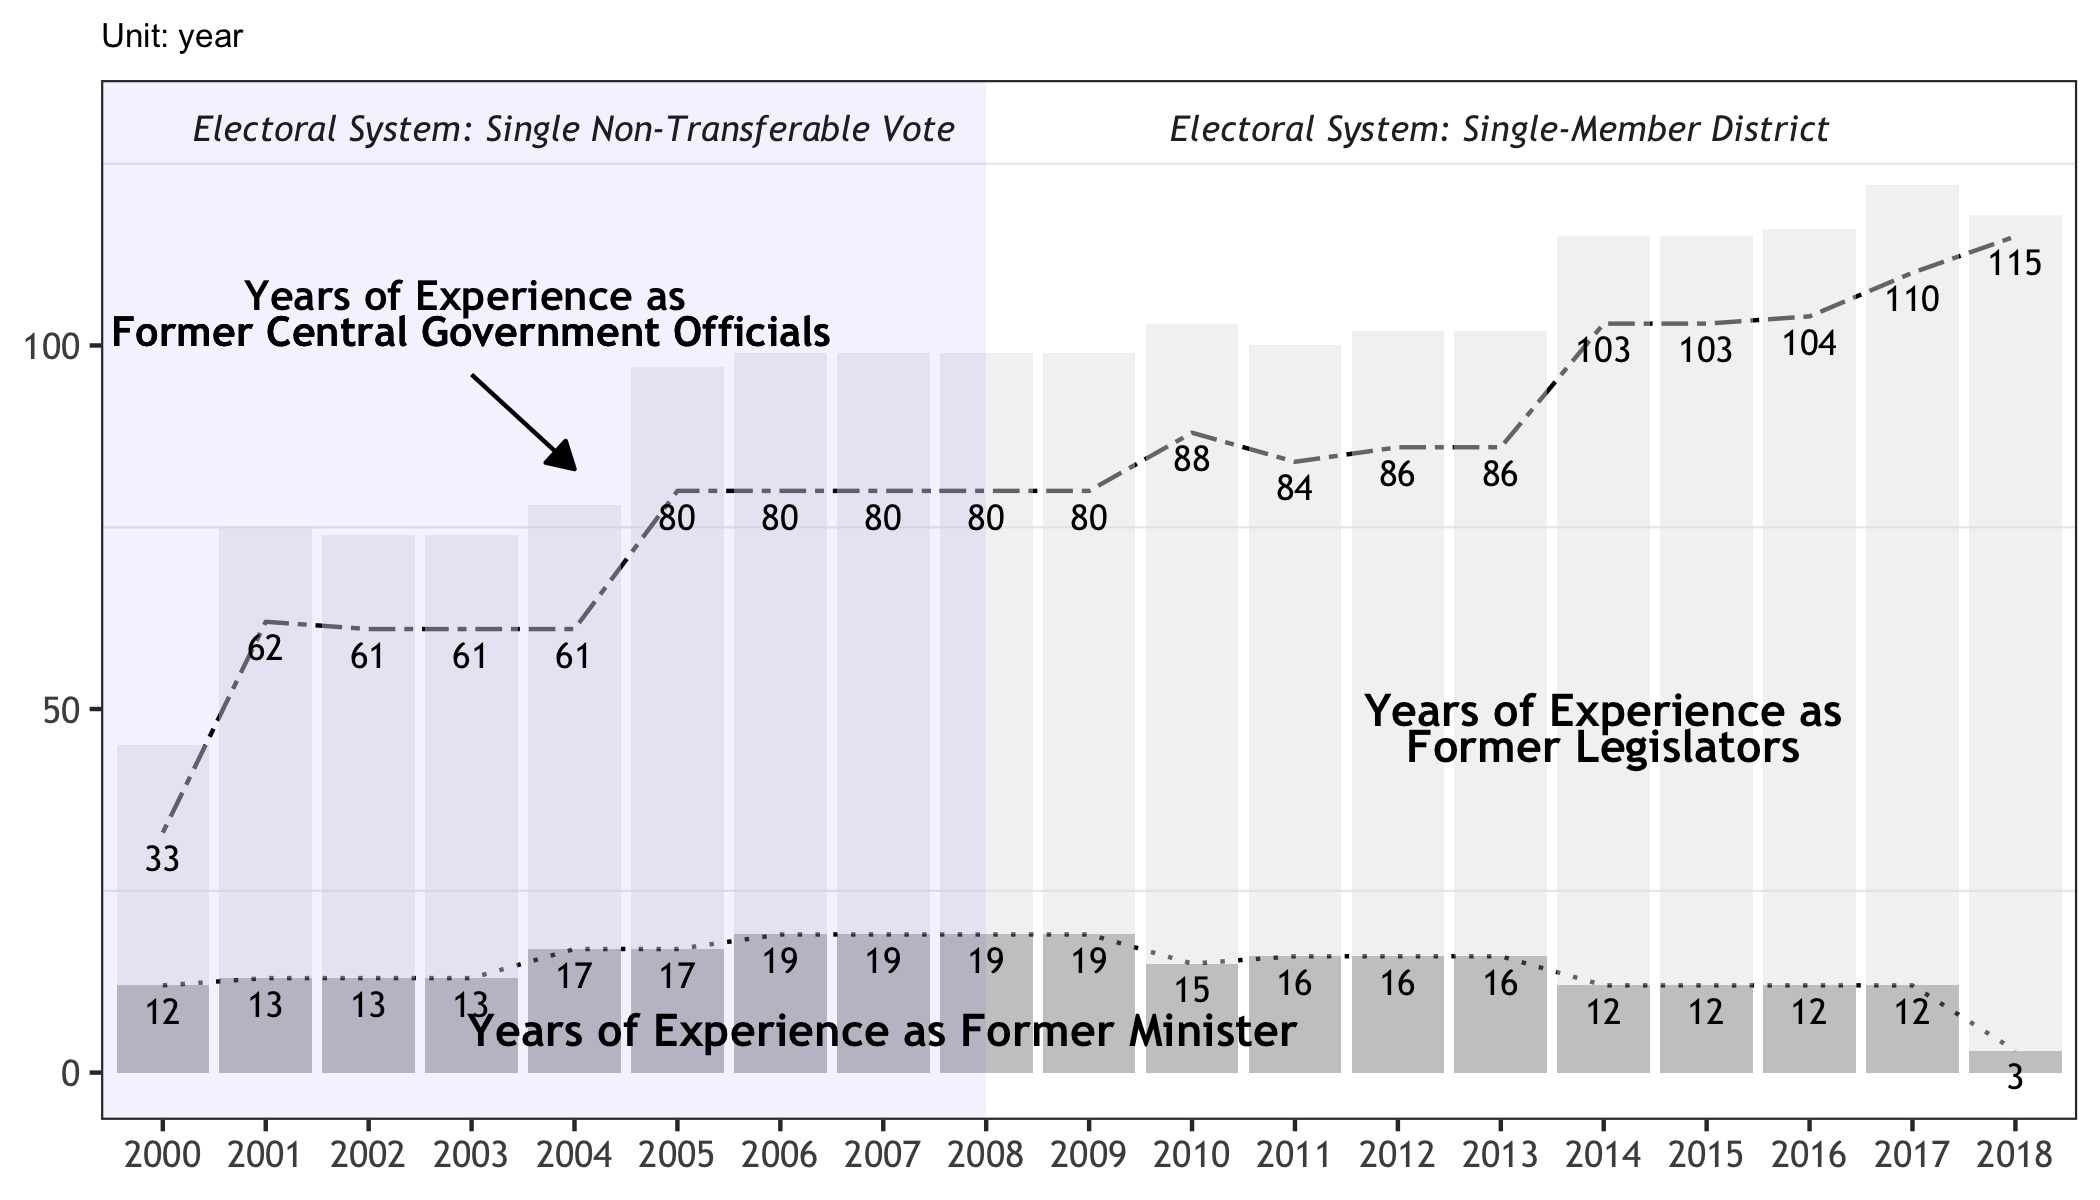
\includegraphics[scale=0.18]{04-Chapter-Four/image/figure1.jpeg}
\end{figure}

\section*{\centering Intergovernmental Transfers and Municipalities}
The municipal government in Taiwan is managed by a mayor elected with a four-year term by the people living in the municipality. Except for the special cities, mayors can continuously be in office if successfully re-elected, which increases incentives for mayors to secure more grant transfers to their municipality. As shown in \autoref{figure2}, the distributions of revenue types point out that approximately more than 40\% of local governments per year rely heavily on the revenue support grant to assist their fiscal expenditure. To secure higher grants, mayors are motivated to seek maximum expenditures. They not only propose projects that fulfil the criteria of receiving grants regulated by the Executive Yuan (the executive branch)  but also reach out to the legislators in an attempt to influence the budgetary decisions. 

Meanwhile, the grant allocation is not distributed following a demographic formula, as the trend varies and frequently fluctuates over time.\footnote{The revenue support grant is discretionarily allocated to municipalities to balance fiscal disparity among the municipalities. Initially aiming for the facilitation of efficient collaborations between inter-government during the development of public infrastructures and designed to be evenly distributed among governments, this grant in practice can be disproportionately distributed among local governments, possibly for specific reasons, such as a closer tie between local governments and the Executive Yuan. These factors have allowed mayors, who have more networks with cabinet officials, to gain privileged access to pork barrels from the central government.} \autoref{figure3} shows the annual distribution of detrended revenue support grants across years, eliminating chronological bias stemming from time-related trends. The enormous variation across all periods reflects that the fiscal revenue allocated by the Executive Yuan is potentially affected by multiple unexplained factors. These patterns ultimately reflected that the grant could be disproportionately more allocated to some municipalities, which the central government's distributive policies favour. 

\begin{figure}[ht]
\begin{centering}
\caption{The Proportions of Fiscal Resources Received by Municipalities\label{figure2}}
\par\end{centering}
\centering{}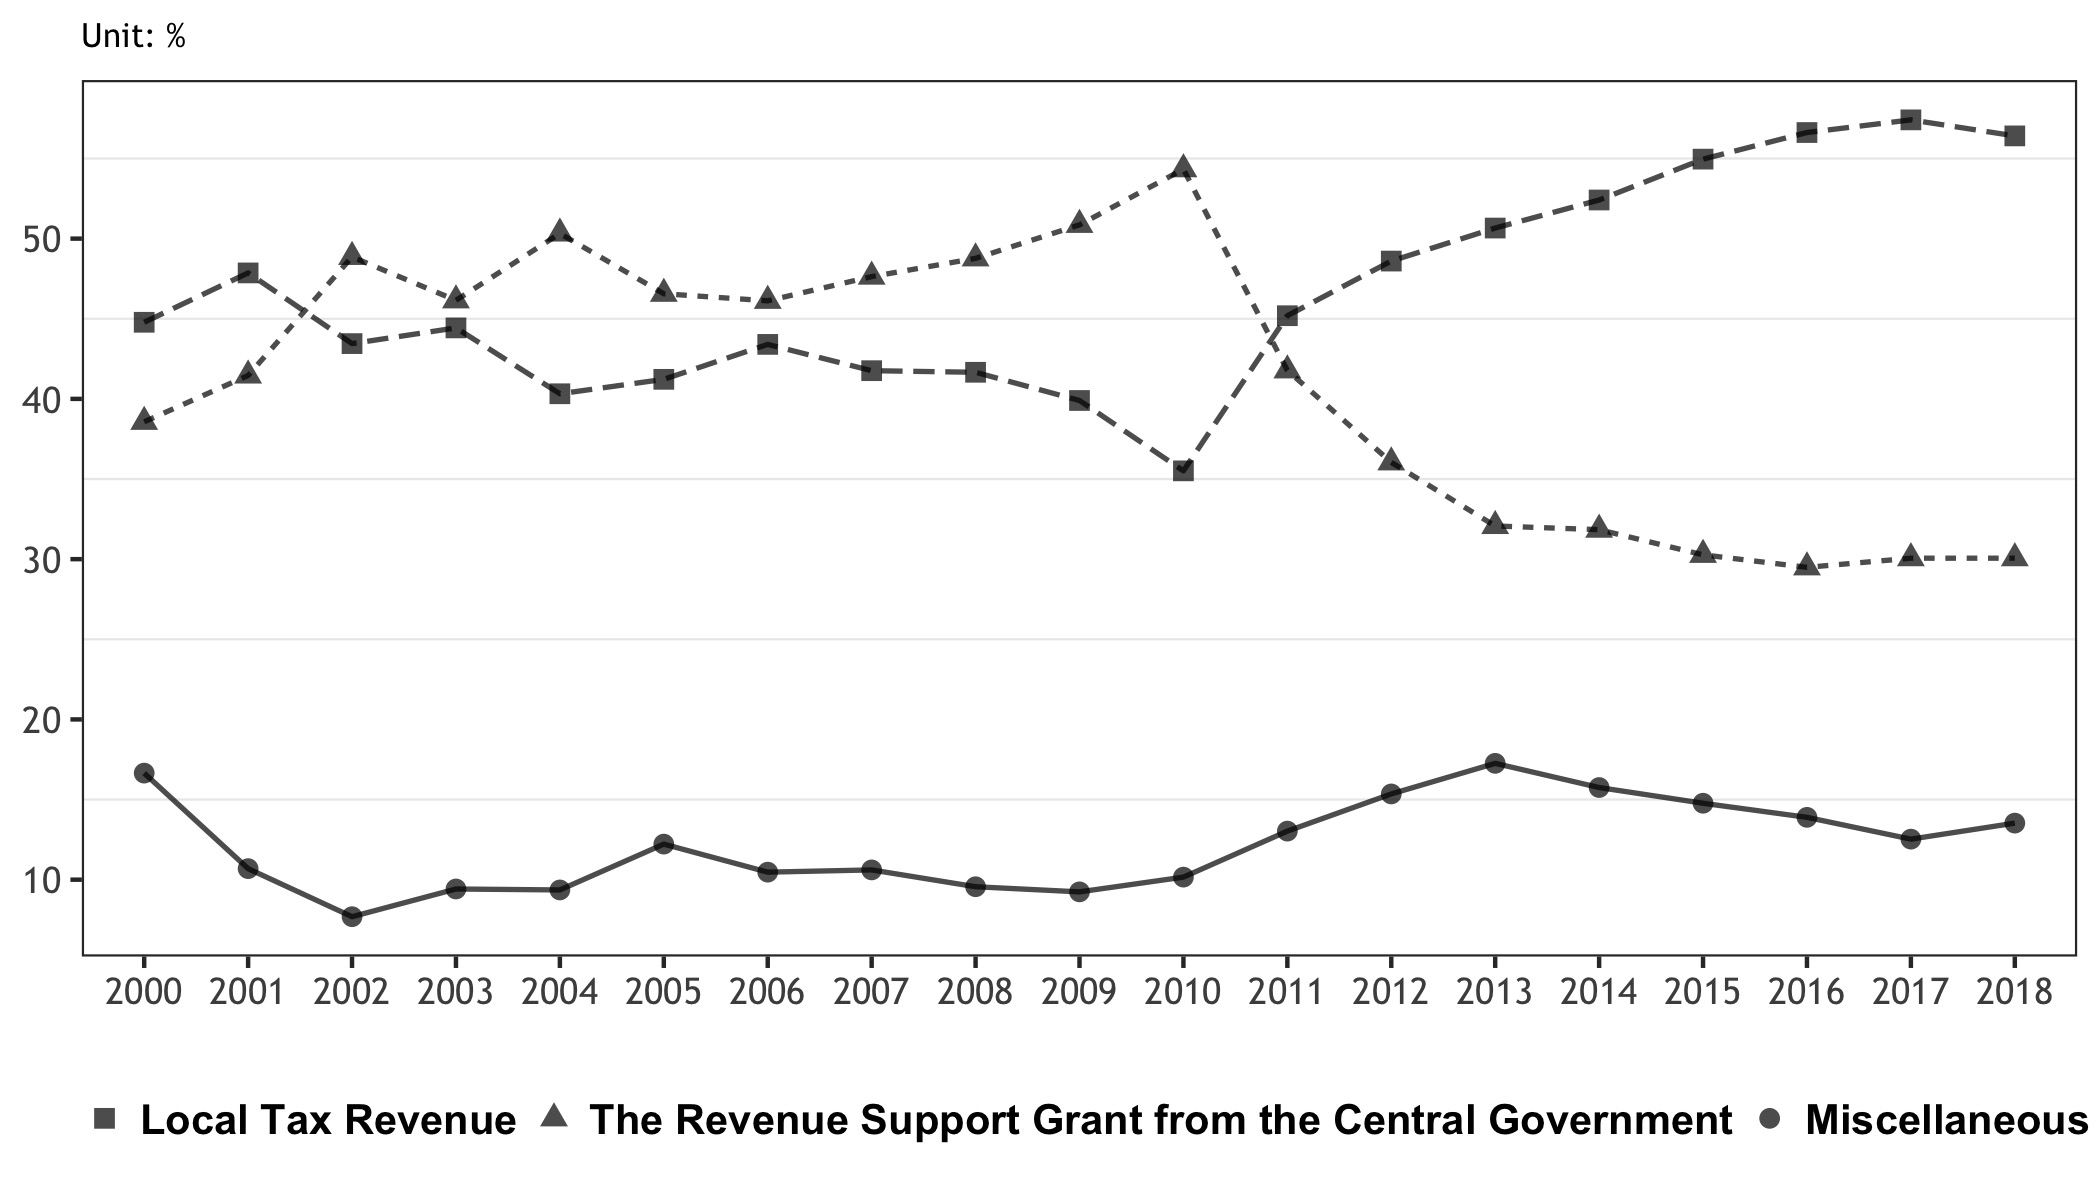
\includegraphics[scale=0.18]{04-Chapter-Four/image/figure2.jpeg}
\end{figure}

Moreover, revenue support grants also can be directly applied to finance the investment and maintenance of local infrastructures, such as public construction and urban development. For example, a municipality's expenditure on bridge and highway reconstruction is self-governed. Unlike other forms of grants, on the one hand, the granter of revenue support grant, the Executive Yuan, is not strictly obliged to obey a specific formula when determining the amount of grant allocated to each municipality. On the other hand, recipient municipalities can unconditionally dictate the money independently. 

\begin{figure}[!htbp]
\begin{centering}
\caption{The Annual Variation of the Detrended Revenue Support Grant\label{figure3}}
\par\end{centering}
\centering{}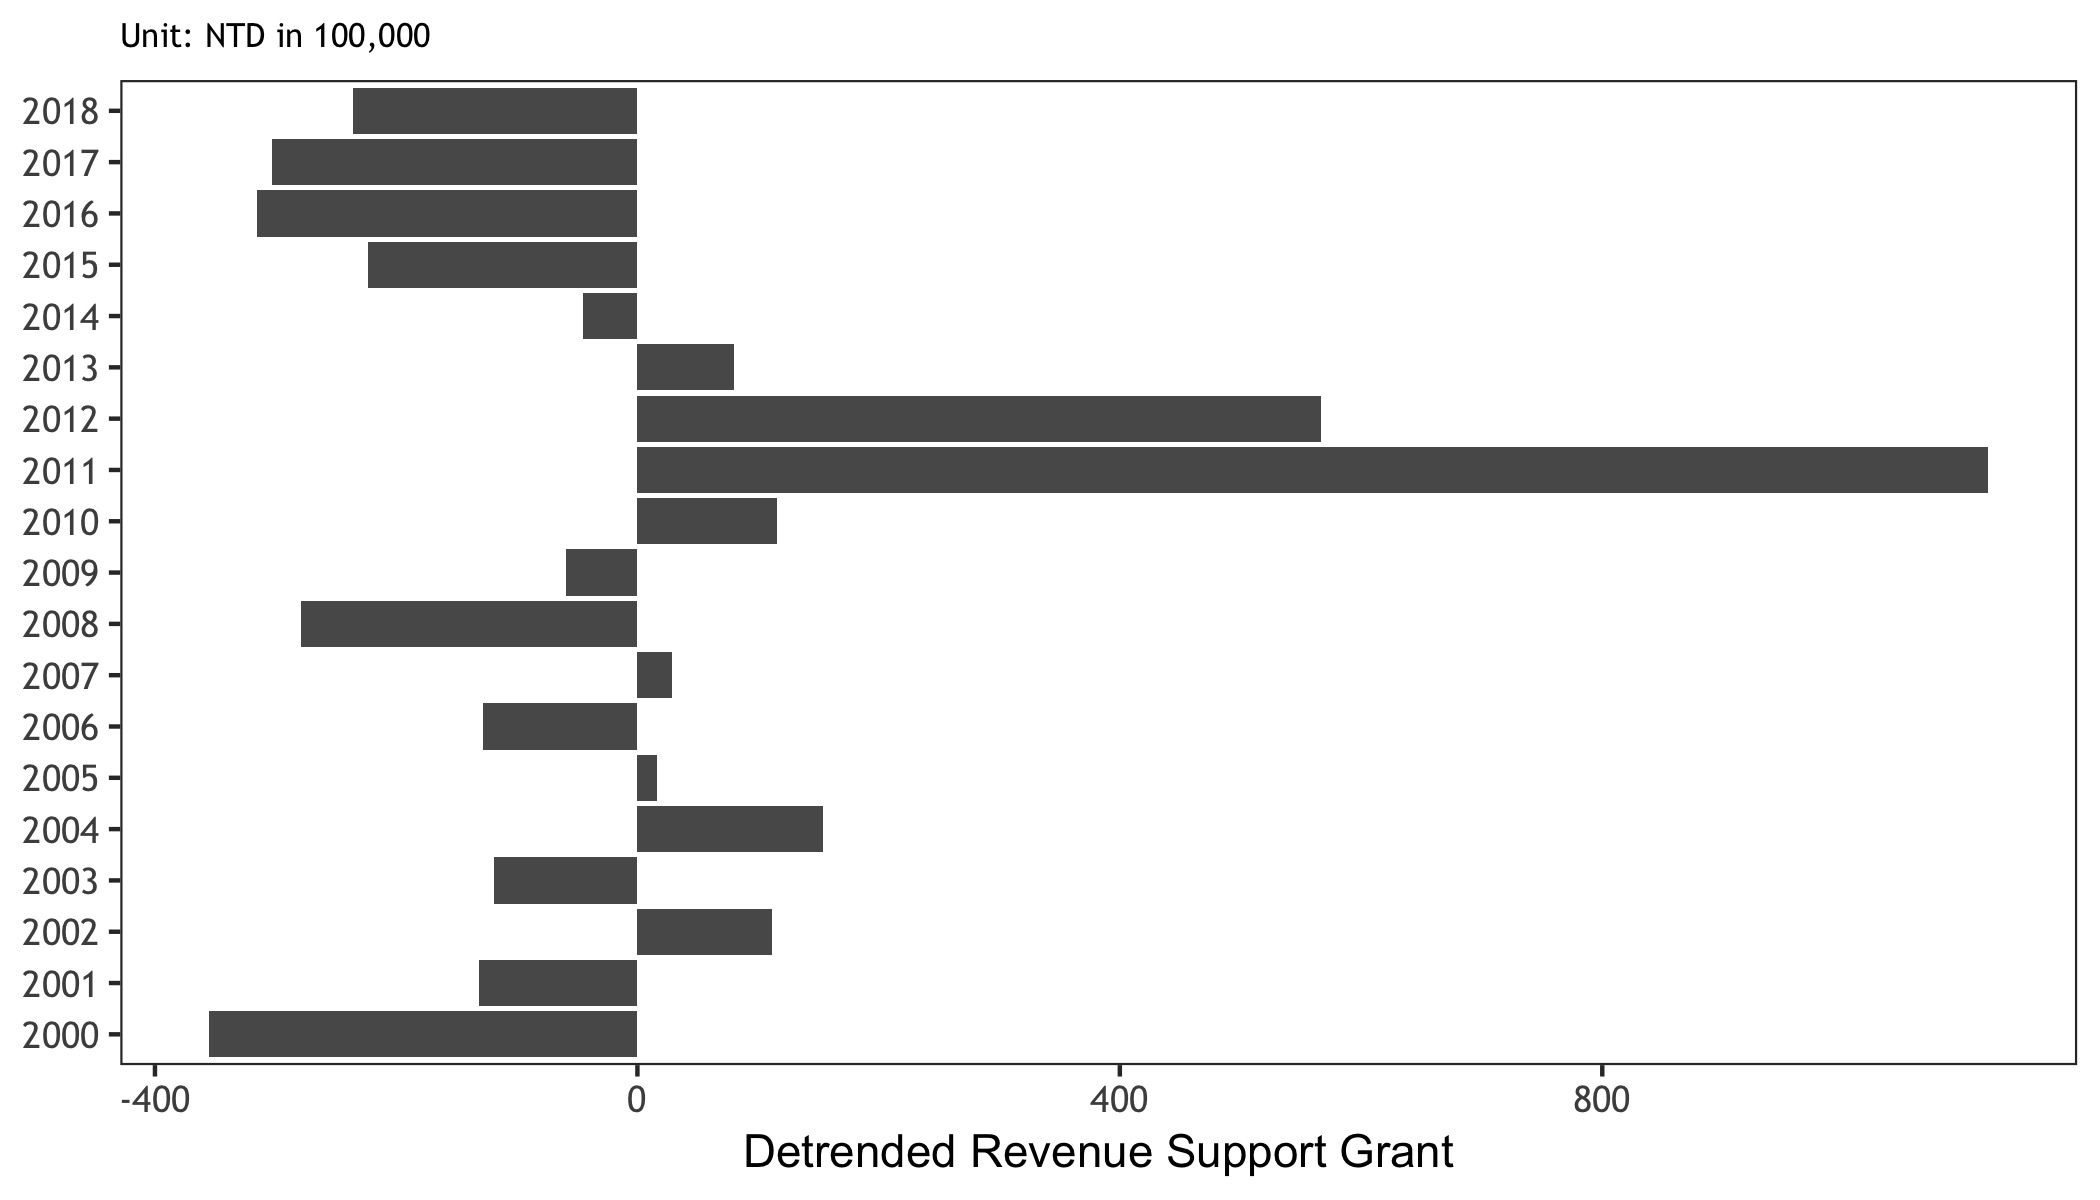
\includegraphics[scale=0.18]{04-Chapter-Four/image/figure3.jpeg}
\end{figure}


\begin{sidewaysfigure}[!htbp]
    \centering
    \begin{subfigure}[t]{0.48\textwidth}
    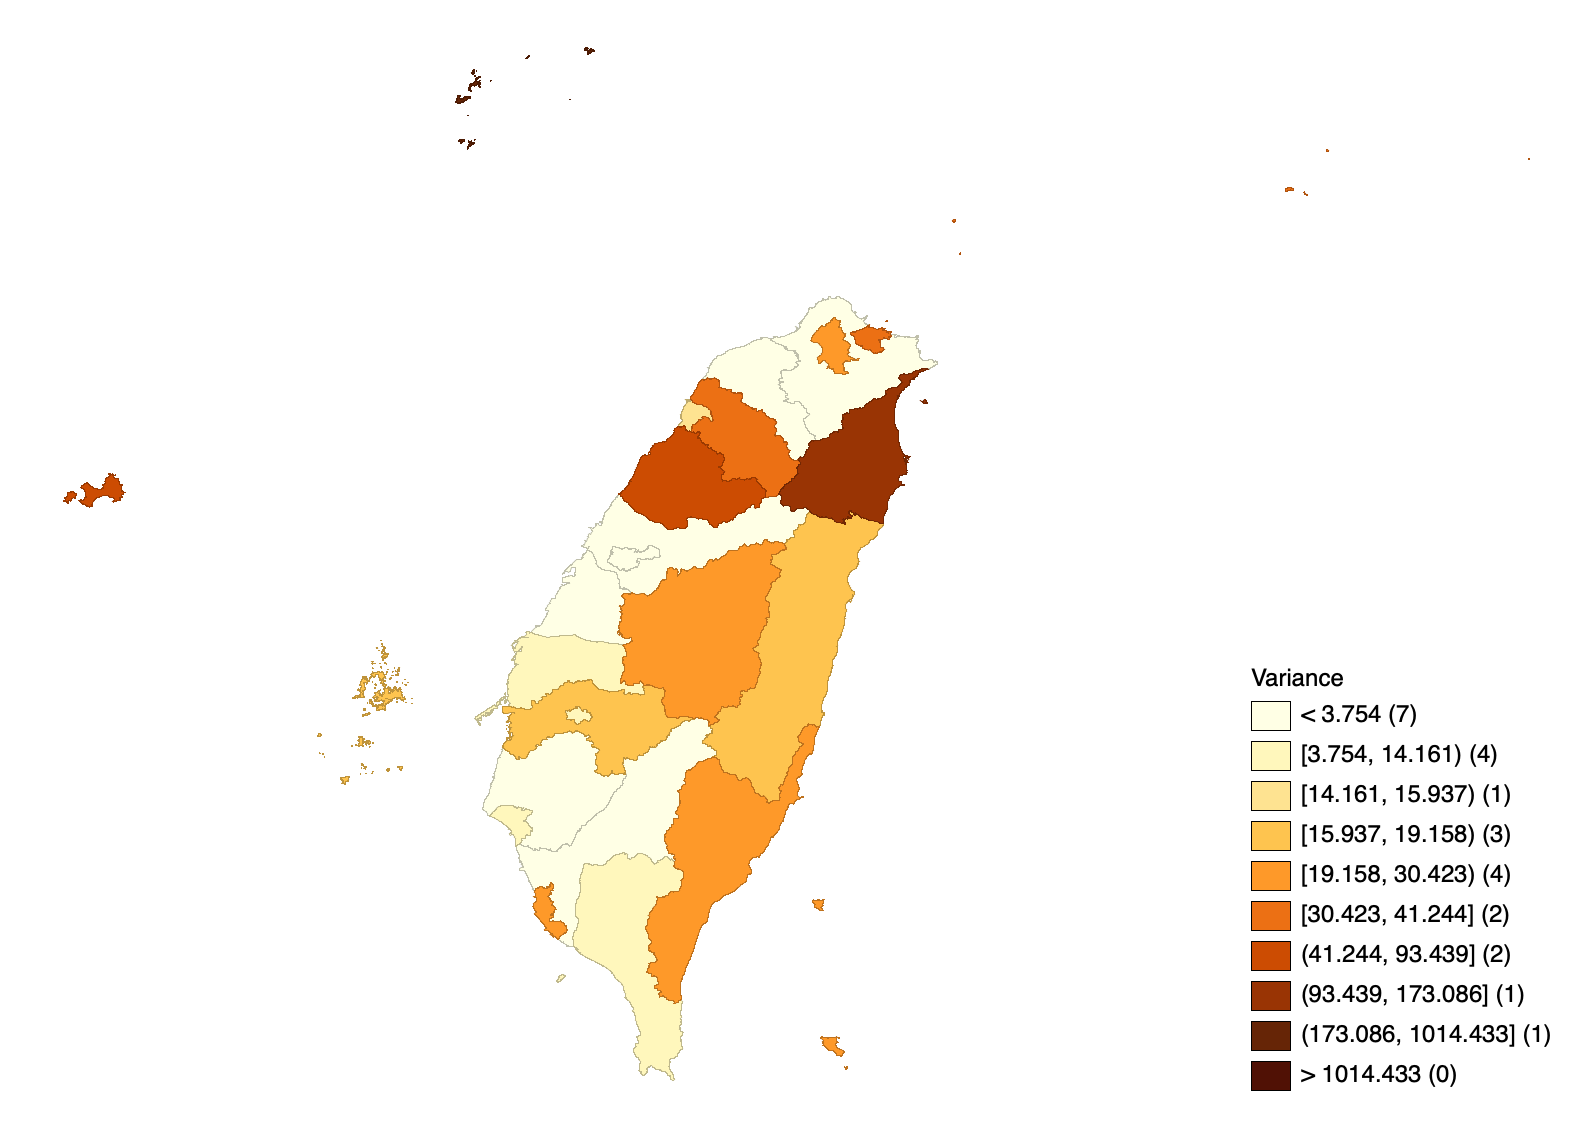
\includegraphics[width=7cm, height=6cm]{04-Chapter-Four/image/figure4-1.png}
    \caption{variance, \textit{pre}-refrom  \\ (No. of municipalities: 25)}
    \label{fig:figure4-1}    
    \end{subfigure}    
    \begin{subfigure}[t]{0.48\textwidth}
    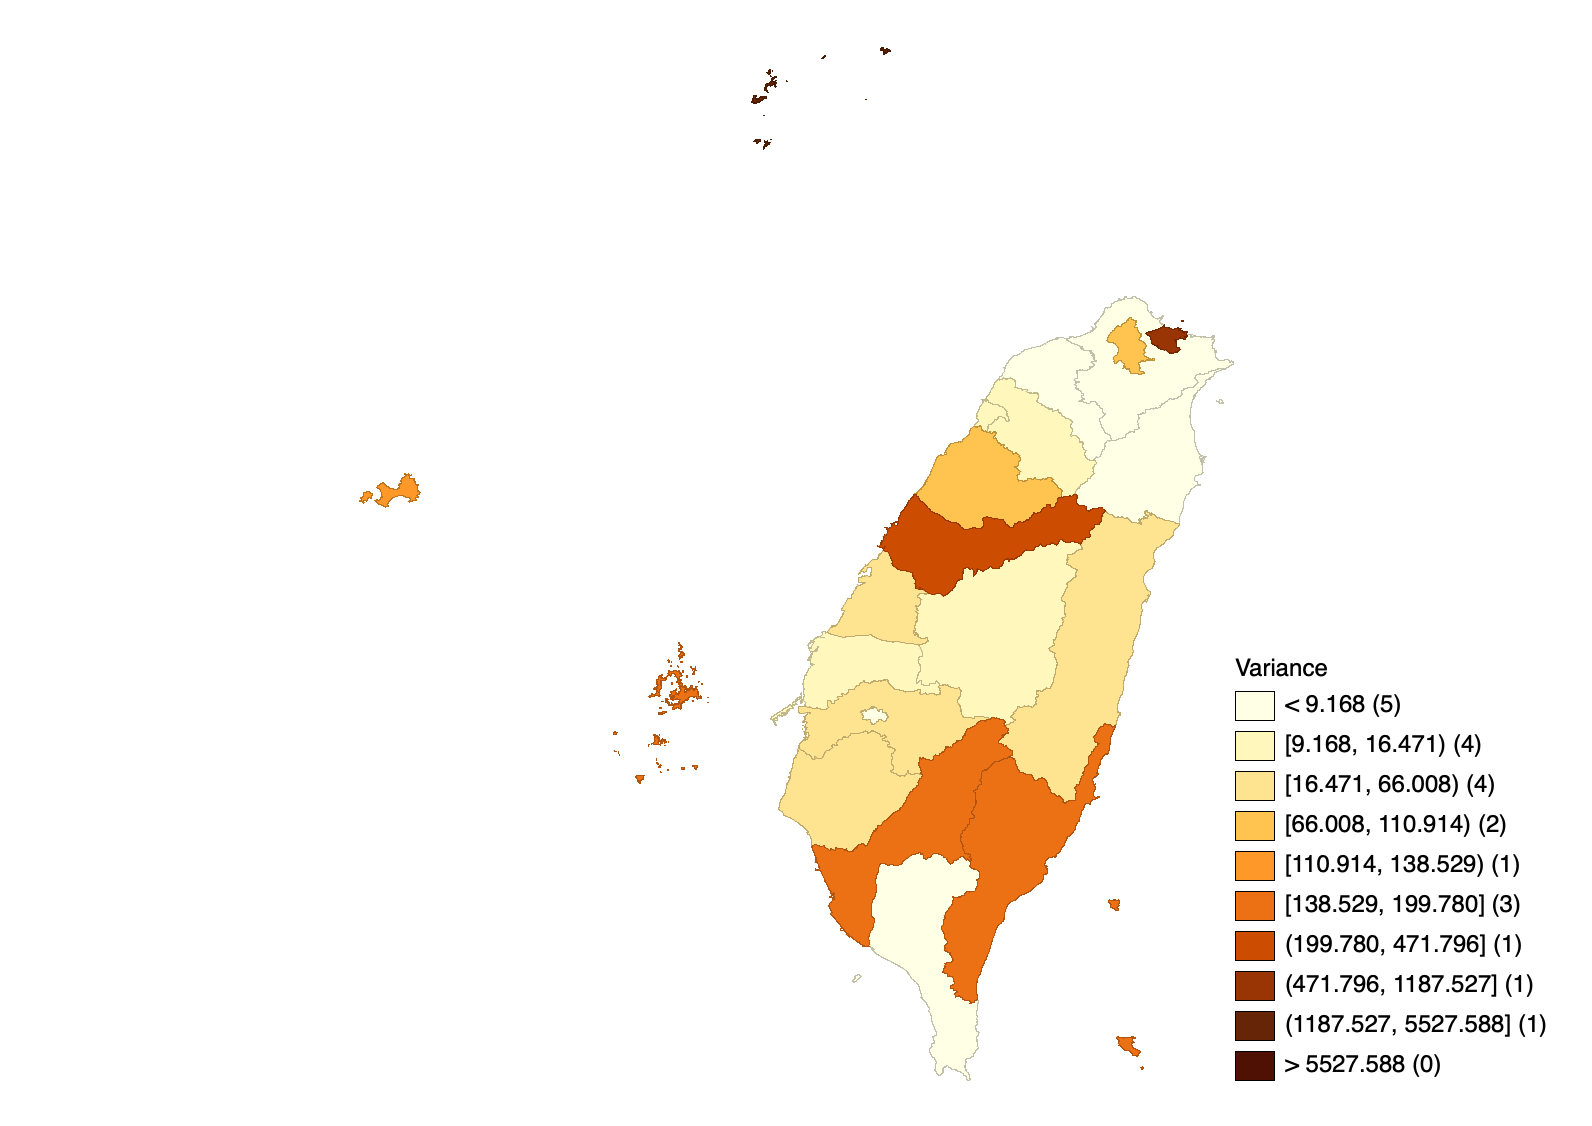
\includegraphics[width=7cm, height=6cm]{04-Chapter-Four/image/figure4-2.png}
    \caption{variance, \textit{post}-refrom \\ (No. of municipalities: 22)} 
    \label{fig:figure4-2}
    \end{subfigure}
    \centering
    \begin{subfigure}[t]{0.48\textwidth}
    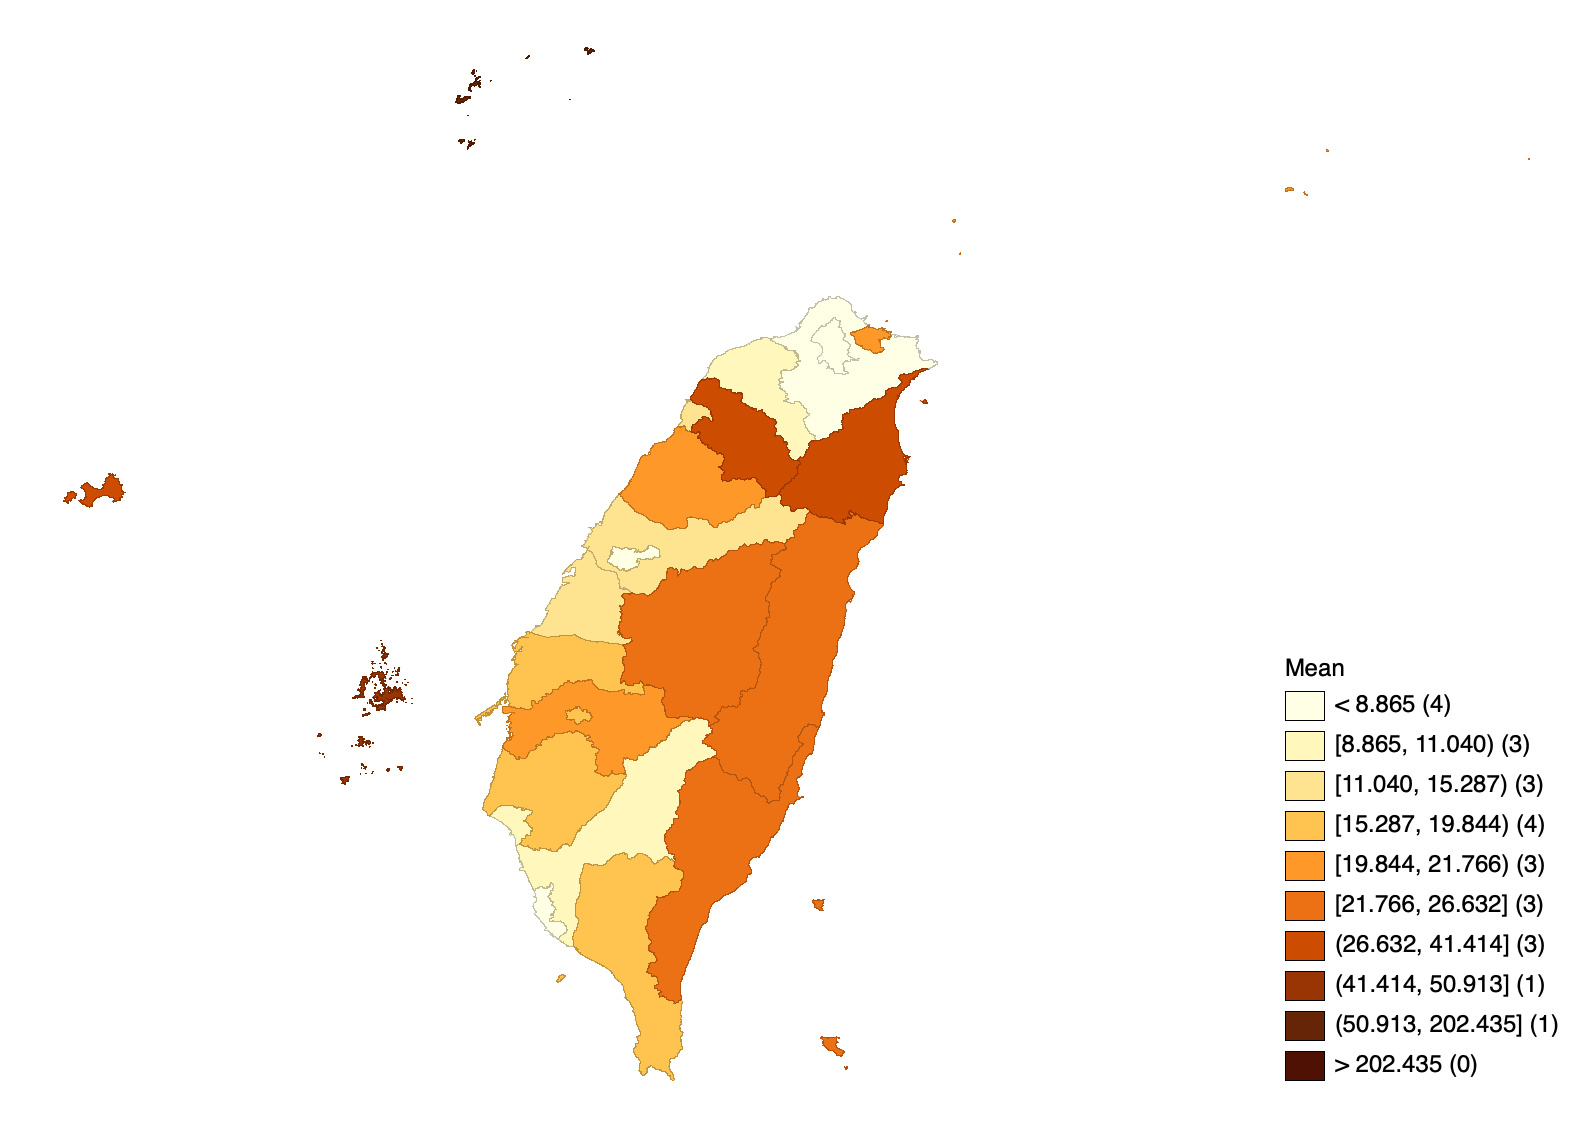
\includegraphics[width=7cm, height=6cm]{04-Chapter-Four/image/figure4-3.png}
    \caption{mean, \textit{pre}-refrom\\ (No. of municipalities: 25)} 
    \label{fig:figure4-3}
    \end{subfigure}    
    \centering
    \begin{subfigure}[t]{0.48\textwidth}
    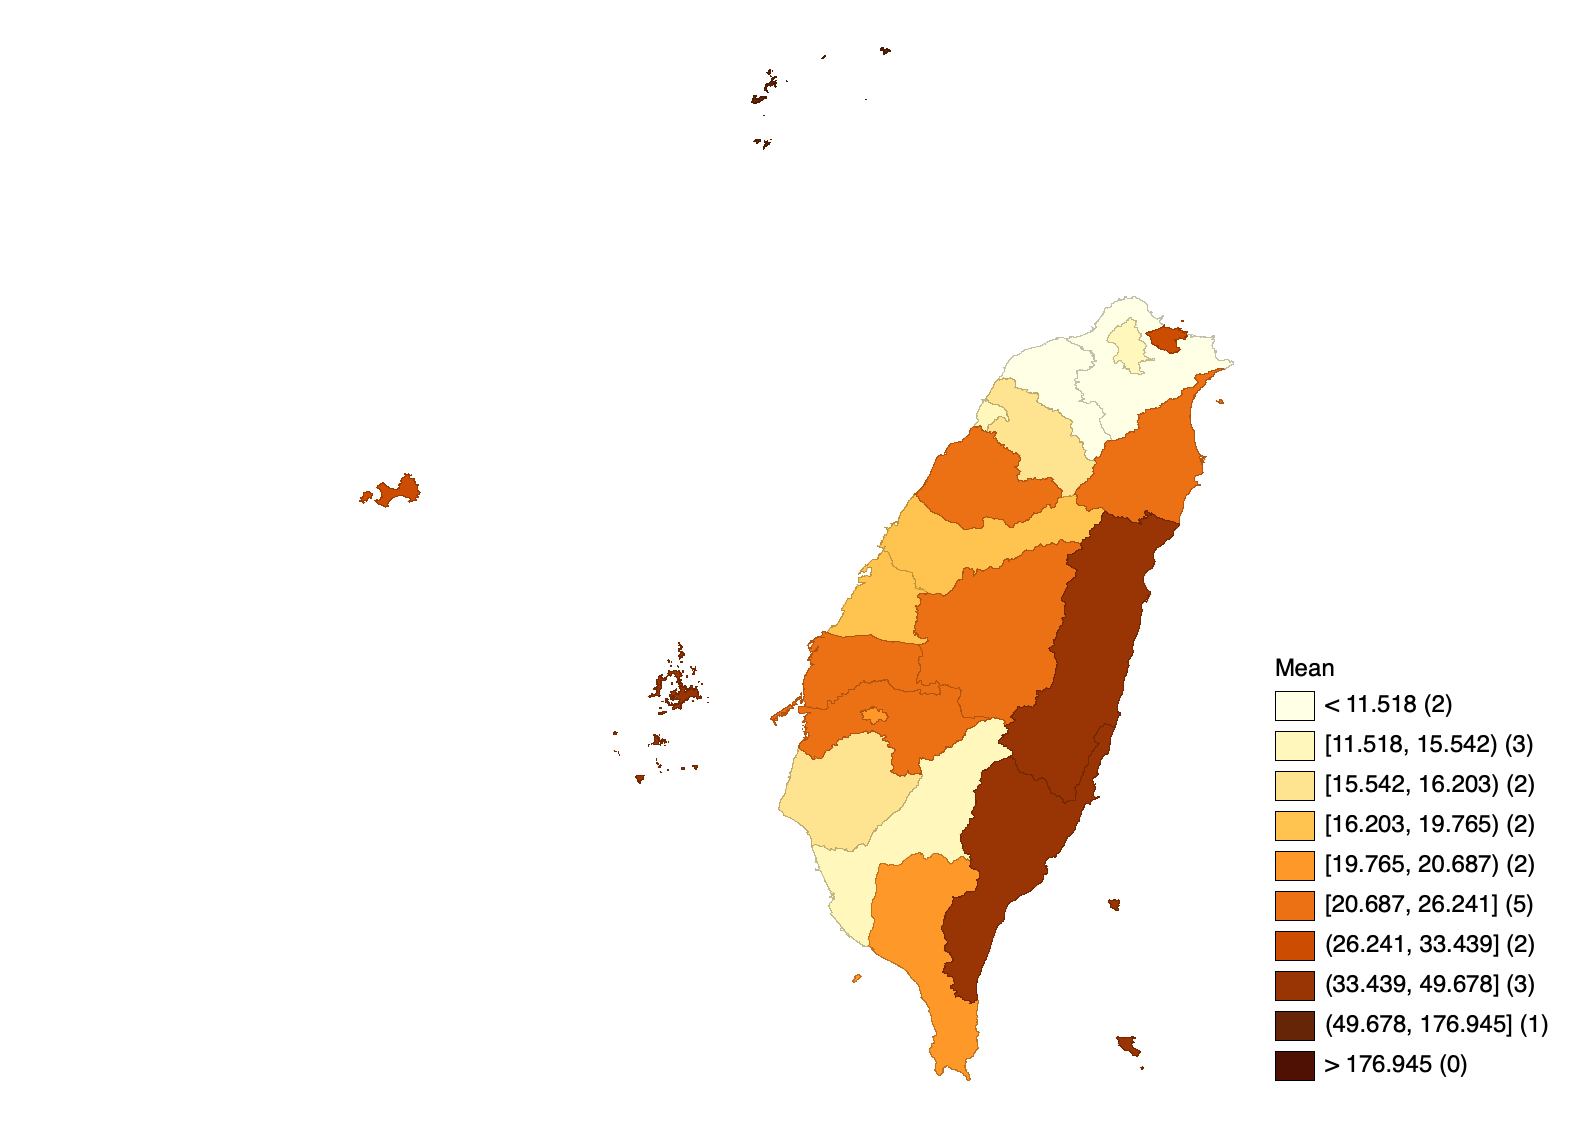
\includegraphics[width=7cm, height=6cm]{04-Chapter-Four/image/figure4-4.png}
    \caption{mean, \textit{post}-refrom \\ (No. of municipalities: 22)} 
    \label{fig:figure4-4}
    \end{subfigure}
    \caption{The Geographical Distribution of the Intergovernmental Transfers, Comparison between Pre- and Post-Reform}\label{figure4} 
\end{sidewaysfigure}

By visualising the patterns of the transfer distribution across municipalities, \autoref{figure4} describes variance and mean variations of the grant allocations per capita within each municipality. \autoref{fig:figure4-1} and \ref{fig:figure4-2} display the variance in grants distributed to each municipality over 2000-2008 (pre-reform) and 2009-2018 (post-reform). The deeper colour represents higher variation in the distribution of the grant. Similarly, \ref{fig:figure4-3} and \autoref{fig:figure4-4} show the average grant distribution allocated to each municipality. In particular, I observe a higher centrality within mid-eastern municipalities. For example, mid-eastern Taiwan always received higher grants, regardless of the merger scheme. According to these patterns, the ruling government potentially allocate to specific municipalities whose mayors are more politically associated with the central government. 

\section*{\centering Research Design}

\subsection*{Data}
To investigate whether mayors exploit their privilege of being aligned with the government party to obtain more grants, I identify each mayor's years of working experience within the congress (the Legislative Yuan) and the executive administration  (the Executive Yuan), and the amount of Revenue Support Grant that each municipal government allocated from 2000-2018.\footnote{The data are obtained from the Directorate General of Budget, Accounting and Statistics, DGBAS. The variables of interest are annually collected at the municipal level, which consists of the percentage of corresponding municipal mayors who previously served in the cabinet, the percentage of mayors formerly elected as legislators and representing the municipality, and whether mayors were once serving as a committee member in the Legislative Yuan. The data set contains each mayor's name and party affiliation, local demographics, and voter turnouts in presidential and mayoral elections (from the Central Election Commission, CEC). The control variables include the unemployment rate (from the Directorate General of Budget, Accounting and Statistics, DGBAS) and demographic information (from National Statistics).} In order to get accurate information regarding mayors' demographics, the data were cross-referenced by corresponding information on Wikipedia, local newspapers, municipalities' websites and the mayor's blog.

In my identification strategy, all ministries, councils and commissions are being comprehensively classified, except for ministers without portfolio who do not actually supervise any particular part of the cabinet in the central government.\footnote{The Executive Yuan, led by a premier and a vice-premier, comprises cabinet ministers (and its vice-ministers) and chairpersons of various councils (and its vice-chairpersons), and several (5-7 seats) ministers without portfolio. The premier (also known as the prime minister) appointed by the president requires no consent of the Legislative Yuan, while the president of the Republic appoints the vice premier and other members in the cabinet upon the recommendation of the premier. In addition to supervising the subordinate organs of the Executive Yuan, the premier must explain administrative policies and report significant policy changes to the Legislative Yuan.} As for the Legislative Yuan, its legislative seats comprise constituency seats that represent the people who live in the municipality, party-list seats that represent various parties, and reserving seats for aboriginals. In the data collection, all legislative seats are considered because the legislature plays a vital role in examining legal bills, treaties, and any general budget proposed by the Executive Yuan.\footnote{The minister includes the Ministry of Interior, Ministry of Foreign Affairs, Ministry of National Defence, Ministry of Finance, Ministry of Education, Ministry of Justice, Ministry of Economic Affairs, Ministry of Transportation and Communications, Ministry of Transportation and Communications, Ministry of Health and Welfare, Ministry of Culture, and Ministry of Science and Technology. The councils and commissions include Agriculture Council, National Development Council, Mainland Affairs Council, Financial Supervisory Commission, Overseas Community Affairs Council, Veterans Affairs Council, Indigenous Peoples Council, Hakka Affairs Council, Public Construction Commission, the Atomic Energy Council, Council for Economic Planning and Development (merged by the National Development Council in 2014); and Research, Development and Evaluation Commission (merged by the National Development Council in 2014). In addition, Independent Regulatory Agencies are incorporated into the classification, such as the Central Bank, Environmental Protection Administration, National Palace Museum, and the Consumer Protection Committee (dissolved in the Executive Yuan as the department of consumer protection in 2012).} 


\subsection*{Operationalisation}

The central government attempts to target key municipalities politically or geographically aligned with the central government. An increasing number of municipalities whose mayors have more experience in the legislature are thought to be distributed higher intergovernmental transfers from the central government. The literature has found the interaction between the fiscal resources distributed to local governments and partisanship that explains what motivates the central government to distribute higher fiscal resources to co-partisan strongholds in India \citep{Keefer2008,Keefer2009}, Argentina and Chile (\citealt{Calvo2004,Luna2010}) and in Mexico (\citealt{Diaz-Cayeros2003,Costa-i-Font2003}).

Thus, electoral pressures encourage the executive government or presidents to be more responsive to constituencies whose legislators are politically aligned with the central government. For example, the federal government is more likely to distribute disproportionately more fiscal spending to electorally important strongholds, particularly those states which are currently presented by governors or legislators from the president's party \citep{Aidt2012, Albouy2013, Kriner2015}. To control for the additional effects transmitted from the president and the legislator's attributes, I include three control variables: (1) whether the mayor's party affiliation is co-partisan with the president (\textbf{co-partisan mayor}); (2) the margin of the victory in terms of vote shares, won by the president during elections (\textbf{\%pres. vote}); and (3) the percentage of a municipality's legislators from the president's party (\textbf{\%co-partisan legislators}).

Thus, the relationship between the geographical allocation of revenue support grants and municipalities' attributes may be interfered with by, for example, municipalities represented by privileged legislators who hold strong agenda-setting positions in the legislature \citep[e.g.,][]{Engstrom2010, Martin2014}. The literature has explained the relationship between members having institutional position and the distribution of particularistic benefits \citep{Lazarus2009,Lee2003,Clemens2015,Balla2002,Lai2013,Luor2004,Luor2000, Berry2010}. Similarly, a positive correlation was found Taiwan municipalities receive disproportionately more central government grants when a legislator has standing committee membership, particularly those who hold committee chairs in powerful committees \citep{Chiu2013,Hsiao2007,Matsuo2012,Lai2013}.

To control the influence of the privileged legislators, I introduce two dummy variables that indicate (1) committee chair status (\textbf{committee chair}) and (2) member in powerful committees (\textbf{power committee}); and the number of sessions that the legislator has served in the congress (\textbf{seniority}).\footnote{I calculate the average seniority, average committee chair, and power committee in each municipality. For example, the seniority of legislators from the same municipality is added up across all local legislators for each year and then divided by the total number of local legislators in the municipality} Because some of the municipal governments are special autonomous cities and are directly controlled by the central government, I include a dummy variable indicating if a municipality belongs to this category (\textbf{special cities}). At the macroeconomic level, the unemployment rate is a measurement of the economic condition of a municipality and, therefore, is potentially relevant to grant allocation (\textbf{\%unemployed)} \citep{Adler1997}.

As indicated above, the distribution of such grants is a feasible proxy for the distribution of particularized benefits because they are disproportionately allocated within different local governments. In the data collection, the revenue support grant is individually identified annually from 2000 to 2018 across all municipalities. \footnote{It is worth noting that Lienchiang, Kinmen and Penghu are excluded from the regression analysis because these municipalities are the least populated and are surrounded by islands near Mainland China. Their grant allocations might potentially follow a different rule. I conduct a series of robustness analyses to check the performance of the outcomes by adding these surrounded islands in the sample to the regression estimation, see \autoref{tab:Robustness-of-Empirical-1} and \autoref{tab:Robustness-of-Empirical-2} in the Appendix \ref{sec:robustness}.} In total, the panel data set is unbalanced with 367 municipality-year observations, which resulted from the dissolution of certain municipalities into their surrounding neighbourhoods during the period.\footnote{\autoref{tab:variable} describes an overview of the independent variable and control variables as well as  the definitions of each variables.}

\subsection*{Estimation Strategy}
The estimation strategy is based on the adoption of panel data methods to test the significance of the coefficient between current mayors who have more previous experience in central government and distributive benefits across the municipalities.\footnote{In regression tables, the estimation of Model (1) is the results for the pooled cross-sectional model which treats the panel data as random samples simply drawn from the whole population, regardless of years. Under the statistical assumption that municipality-specific effects for different years are constant and time-specific effects for different municipalities are also $IID$, the Model (3) and Model (4) show the results of the models using the Fixed Effects by specifying the disturbance term $ \mu_{it}$, municipality dummies and year dummies to capture fixed and time-varying effects, respectively. The municipality-effect estimators in columns 3 yield consistent estimates under the assumption that some municipalities may potentially have strong connections which increase the municipalities' possibility of being given such a good share of the grant from the central government. For example, municipalities having a higher proportion of senior legislators or legislator holding privileged positions in the committee get themselves a great bargaining position in budgetary allocation. Likewise, time-varying effects could also be an issue if, for example, poor municipal governments that have been suffering from higher unemployment rates intermittently for many years are likely to be allocated more grants than other municipal governments. In order to compare the potentially different results of the estimation, column 2 of the table also includes a Random Effect model to confirm the robustness of the findings, under a different assumption from the Fixed Effect model, that the municipality-specific effects for different years are $IID$, similarly, time-specific effects from different municipalities are also $IID$.} In equation (1), $mayor_{i,t}$, as one of variables of interest indicates the past experience of the $i-th$ local government's mayor has in the central government at time $t$. Theoretically, if a mayor has more relative experience in the central government, with respect to other mayors, the current, say at time $t$, local government is more likely to receive more grants from the central government, that is, the extra experience plays a part in helping the local government (i.e. mayor) obtain a higher sharing of pork barrel benefits in following year ${t+1}$. 

In light of the municipal merge scheme after the electoral reform during the sample period, the value of experience does not imply same level of competitiveness in applying for central governmental grants in different years. Due to a variation in the total number of local governments existing across time, $mayor_{i,t}$ is adjusted by its municipal numbers to penalise potential effects of the mayors' experience in comparison to another at a different time (year) with lesser numbers of municipalities. More specific, $mayor_{i,t}$ is calculated as years of the central government experience of $i-th$ mayor, with respect to the total number of local government at $t$: $\Sigma_{1}^{T=t}\epsilon_{iT}$/$N_t$, where $\epsilon_m{}_n$ is the cumulative absolute experience of $m-th$ mayor has at time $n$, and $N_t$ is the total number of local governments. Notably, only the experience as Executive Yuan minister and Legislative Yuan legislator is counted as central government experience.

Based on the notations described above, the general model can be expressed
as Model (1):

\begin{equation} \ensuremath{y_{i,t+1}^{grant}}=\ensuremath{\beta_{A}{\Delta mayors}_{i,t} + X_{i,t}\gamma + \alpha_{i} + \delta_{t} + \varepsilon_{i,t}},\end{equation}

where $y_{i,t+1}^{grant}$ is the (log of) Revenue Support Grant per capita in New Taiwan Dollars (thousand) allocated to the $i-th$ local government by the Executive Yuan for period $t+1$; $\Delta mayor_{i,t}$ is the explanatory variable of interest, as explained above; the row vector, $X_{i,t}$, contains control variables isolating various effects from the legislature, the president and its own demographics, with
a column of corresponding coefficients $\gamma$. 


\begin{table}[!htbp]
\caption{The Estimation of Revenue Support Grant and the Mayor with Years of Experience as the Central Government Officials
\label{tab:table1}}
\centering{}%
\scalebox{0.85}{

\begin{threeparttable}

\begin{tabular}{lcccc}
\toprule 
\multicolumn{5}{l}{Dependent Variable:}                                                                  \\
\multicolumn{5}{l}{\textbf{log (Revenue Support Grant)}}                                                 \\
\midrule
                                        &  Model (1)      & Model (2)       & Model (3)  & Model (4)     \\
\midrule
$\Delta{\textbf{\textit{mayors}}}$      &  0.455$^{***}$& 0.456$^{***}$ & 0.473         & 0.324          \\
                                        & (0.152)       & (0.167)       &(0.170)        &(0.149)         \\
\textbf{seniority}                      &  0.005        &  0.036        & 0.042         & 0.088          \\
                                        & (0.216)       & (0.178)       &(0.179)        & (0.214)        \\
\textbf{power committee}                &  0.657$^{***}$&  0.128        & 0.095         & 0.523$^{***}$  \\
                                        & (0.117)       & (0.103)       & (0.104)       & (0.120)        \\
\textbf{committee chair}                & 0.114         & 0.033         & 0.025         & 0.215          \\
                                        & (0.188)       &(0.151)        & (0.151)       &(0.181)         \\
\textbf{mayoral election}               & 0.018         & 0.023         & 0.025         & 0.386$^{***}$  \\
                                        & (0.055)       &(0.044)        & (0.044)       & (0.104)        \\
\textbf{\%pres. vote}                   & 0.329         & 0.094        & 0.057         & 0.021           \\
                                        & (0.226)       & (0.182)       & (0.183)       & (0.251)        \\
\textbf{co-partisan legislator}         & 0.221$^{***}$ & 0.195$^{***}$ & 0.188$^{***}$& 0.100           \\
                                        & (0.050)       & (0.041)       & (0.041)       & (0.133)        \\
\textbf{\%unemployed}                   & 7.721$^{**}$  & 5.847$^{***}$ & 5.781$^{***}$& 12.493          \\
                                        & (3.511)       & (2.835)       & (2.851)       & (8.288)        \\
\textbf{special cities }                & 7.721$^{***}$ & 0.096         & 0.092         & 0.738$^{***}$  \\
                                        & (0.057)       & (0.117)       & (0.131)       & (0.054)        \\
\textbf{constant}                       & 1.956$^{***}$ & 2.089$^{***}$ &               &                \\
                                        & (0.205)       & (0.196)       &               &                \\
\midrule 
\textbf{No. of observations}            & 367           & 367           & 367           & 367            \\
\textbf{adjusted \textit{R}$^{2}$}      & 0.462         & 0.190         & 0.146         & 0.449          \\
\textbf{model types}                    & Pooled OLS    & RE            & FE            & FE             \\
\textbf{fixed effects  by municipality} &               &               & $\checkmark$  &                \\
\textbf{fixed effects by year}          &               &               &               & $\checkmark$   \\
\midrule
\end{tabular}
\begin{tablenotes}
Note: *\(p<0.10\),** \(p<0.05\), *** \(p<0.01\). Robust standard errors in parentheses.  Standard errors are clustered by the municipality.
\end{tablenotes}
    \end{threeparttable}
    }
\end{table}

\section*{\centering Findings}
I first investigate how prior political careers in the ministries and the Legislative Yuan increase mayors' municipalities to obtain higher Revenue Support Grant. \autoref{tab:table1} illustrates the initial findings of the models analysing the grant allocated to municipalities having more current mayors who previously served in the central governments as the dependent variable. All models in \autoref{tab:table1} show support for the expectation that mayors who used to work as government officials or legislators are more likely to acquire a larger share of the grants. The correlation is statistically significant in each model, with a 95\% confidence interval in consistently positive ranges.\footnote{see each regressions of marginal effects in Appendix \ref{fig:margin-model} } Thus, I find consistent empirical evidence in favour of theoretical expectation.


\begin{table}[!htbp]
\caption{The Estimation for the Mayor with Years of Experience \\ as Legislators and Ministers\label{tab:table2}}
\centering{}{\small{}}%
\scalebox{0.85}{
 \begin{threeparttable}

\begin{tabular}{lcccc}
\toprule 
\multicolumn{5}{l}{Dependent Variable:}                                                                          \\
\multicolumn{5}{l}{\textbf{log (Revenue Support Grant)}}                                                         \\
\midrule
                                         &  Model (1)      & Model (2)       & Model (3)  & Model (4)            \\
\midrule
$\Delta{\textbf{\textit{ministers}}}$    & 0.242           & 0.418         & 0.586         & 0.019               \\
                                         & 0.363)          & 0.407         & 0.418         & 0.346               \\
$\Delta{\textbf{\textit{legislators}}}$  & 0.464$^{***}$   & 0.459$^{***}$ & 0.465$^{***}$ & 0.339               \\
                                         & 0.153           & 0.169         & 0.173         & 0.150               \\
\textbf{seniority }                      &  0.007          & 0.036         & 0.041         & 0.094               \\
                                         & (0.217)         & (0.178)       & (0.180)       & (0.214)             \\
\textbf{power committee}                 & 0.658$^{***}$   & 0.128         & 0.095         & 0.658$^{***}$       \\
                                         & (0.117)         & (0.103)       & (0.104)       & (0.120)             \\
\textbf{committee chair}                 & 0.110           & 0.032         & 0.025         & 0.210               \\
                                         & (0.188)         & (0.151)       & (0.152)       & (0.181)             \\
\textbf{mayoral election}                & 0.018           & 0.023         & 0.024         & 0.389$^{***}$       \\
                                         & (0.055)         & (0.044)       & (0.044)       & (0.104)             \\
\textbf{co-partisan mayors}              & 0.039           & 0.044         & 0.048         & 0.039               \\
                                         & (0.050)         & (0.041)       & (0.042)       & (0.049)             \\
\textbf{\% mayor vote}                    & 0.855$^{***}$   & 0.744$^{***}$ & 0.742$^{***}$ & 0.715$^{***}$       \\
                                         & (0.188)         & (0.162)       & (0.163)       & (0.183)             \\
\textbf{\% pres. vote}                    & 0.318           & 0.091         & 0.064         & 0.043               \\
                                         & (0.227)         & (0.184)       & (0.185)       & (0.252)             \\
\textbf{co-partisan legislator}          & 0.221$^{***}$   & 0.196$^{***}$ & 0.187$^{***}$ & 0.102               \\
                                         & (0.050)         & (0.041)       & (0.041)       & (0.133)             \\
\textbf{\% unemployed}                    & 7.725$^{***}$   & 5.834$^{***}$ & 5.820$^{***}$ & 12.429              \\
                                         & (3.514)         & (2.842)       & (2.858)       & (8.288)             \\
\textbf{special cities }                 & 0.692$^{***}$   & 0.093         & 0.090         & 0.704$^{***}$       \\
                                         & (0.067)         & (0.118)       & (0.131)       & (0.064).            \\
\textbf{constant}                        & 1.963$^{***}$   & 2.091$^{***}$ &               &                     \\
                                         & 0.206           & 0.197         &               &                     \\
\midrule 
\textbf{No. of observations}            & 367             & 367           & 367           & 367                 \\
\textbf{adjusted \textit{R}$^{2}$}      & 0.461           & 0.188         & 0.144         & 0.449               \\
\textbf{model types}                    & Pooled OLS      & RE            & FE            & FE                  \\
\textbf{municipality fixed effects }    &                 &               & $\checkmark$  &                     \\
\textbf{fixed effects by year}             &                 &               &               & $\checkmark$        \\
\midrule
 \end{tabular}
     \begin{tablenotes}
     Note: * \(p<0.10\),** \(p<0.05\), *** \(p<0.01\). \\ Robust standard errors in parentheses. Standard errors are clustered by municipality. Hausman test\ensuremath{\chi}2 (12)= 13.115 \ensuremath{p}-value = 0.3608 rejects the null hypothesis 
     \end{tablenotes}
     \end{threeparttable}
     }
\end{table}

Among control variables, \textbf{power committee} is significantly positive in Model (1) Model (4) but insignificantly in columns 2 and 3. However, the estimation of the Hausman test indicates that unobserved errors among the variables are not correlated with the regressions (at p = 0.20, $\chi$ =13.42). The municipalities having privileged legislators serving in powerful committees do not directly influence the allocation of the grant transferred. Likewise, the result of \textbf{seniority} in \autoref{tab:table2} is not consistently associated with the distribution of particularistic goods. In other words, the municipalities represented by most senior legislators do not significantly increase a municipality to obtain a great large share of grants.

In addition, the higher the percentage of vote share a mayor wins during previous elections, the more grants a municipality obtains from the executive government. As mentioned above, the result of the Hausman test, \textbf{\%pres.vote} in Model (2) is significantly correlated with the amount of the grant distribution, which indicates that a high percentage of presidential vote share seems to increase the municipality to obtain government resources. On the other hand, \textbf{\%mayor vote} is consistently correlated with the distribution in grant transfers, and the confidence interval in each model consistently show positive ranges at a given level of confidence.

As to demographic variables, municipalities with higher unemployment rates tend to benefit more from revenue support grants from the central government. \textbf{special cities} in the main result is not statistically significant, indicating that there are no significant differences between them. The autonomous municipalities directly-controlled by the Executive Yuan are not awarded significantly higher grants because of their status. 

\subsection*{The Inequality Allocation of Intergovernmental Transfers}

The core questions are, is it necessary that by the mayor serving more years  in the central government, that the municipality is given more leverage in obtaining grants? Does the number of terms that a mayor has served as a minister give a municipality more leverage in obtaining grants? Does having experienced mayors who previously served as a legislator facilitate a local government in gaining a larger share of the grants? To investigate these research questions, I decompose $\Delta mayors_{i,t}$ in to two sub-categories, $\Delta minister_{i,t}$ and $\Delta legislator_{i,t}$ indicating the experience of serving as $\Delta mayors_{i,t}$ in the Executive Yuan and $\Delta legislator_{i,t}$ in the Legislative Yuan, respectively. 

\autoref{fig: figure5} displays the case where the mayor's prior experience in the central government is decomposed into two subcategories, (a) and (b). The decomposition of an explanatory variable allows us to further examine the extent to which the contribution of central government experience comes from the experience as former minister in Executive Yuan and as former legislator in Legislative Yuan, separately. Naturally, the regression model can be extended and rewritten as 

\begin{equation} \ensuremath{y_{i,t+1}^{grant}}=\ensuremath{\beta_{1}{\Delta minister}_{i,t} + \beta_{2}{\Delta legislator}_{i,t} + X_{i,t}\gamma + \alpha_{i} + \delta_{t} + \varepsilon_{i,t}}.\end{equation}

In particular, this decomposition is motivated by the following three reasons. First, this decomposition allows us to test individually, if a municipality whose mayor has experience as a legislator in central government facilitates it to significantly obtain more government resources, especially the revenue support grant, as well as if a municipality whose mayor has experience as a minister gives it relative advantage in obtaining governmental funding. Secondly, by comparing the corresponding estimates from regressions, I can directly see which of the above experience in central government is more effective in helping the municipality get allocated more resources. Finally, existing studies only focus on either the influence of the legislature side or the impact of the presidency side. By analysing mayors' past experience in the legislature and ministries, the estimation comfortably includes the effect from both sides, plus the impact of mayors in the process of resource allocation. This means, the estimation has the potential to evaluate the inter-governmental (from the central government to local municipalities) resource transfer, under the influence of the Legislative Yuan and Executive Yuan, simultaneously. 

\autoref{tab:table2} illustrates the estimation results of regression equation (2). Hausman test is in favour of Model (2), Random Effect. As can be seen in column 3, a municipality whose current mayor has more experience as a legislator receives more revenue support grant transferred, with 95\% confidence level. The main results in column 3 are robust to different estimation methods and different sets of control variables. Though economically significant, mayors' experience in ministries is not statistically significant in explaining the change in the grants received by municipalities. Therefore, the finding suggests that mayors' experience as legislators is the primary explanation for the variation in resources distribution among municipalities.

\begin{figure}[ht]
\begin{singlespace}
\begin{centering}
\caption{Mayor's Average Years of Experience in Legislative Yuan and Executive Yuan\label{fig: figure5}}
\par\end{centering}
\end{singlespace}
\begin{tabular}{cc}
(a) The Legislative Yuan & (b) The Executive Yuan\tabularnewline
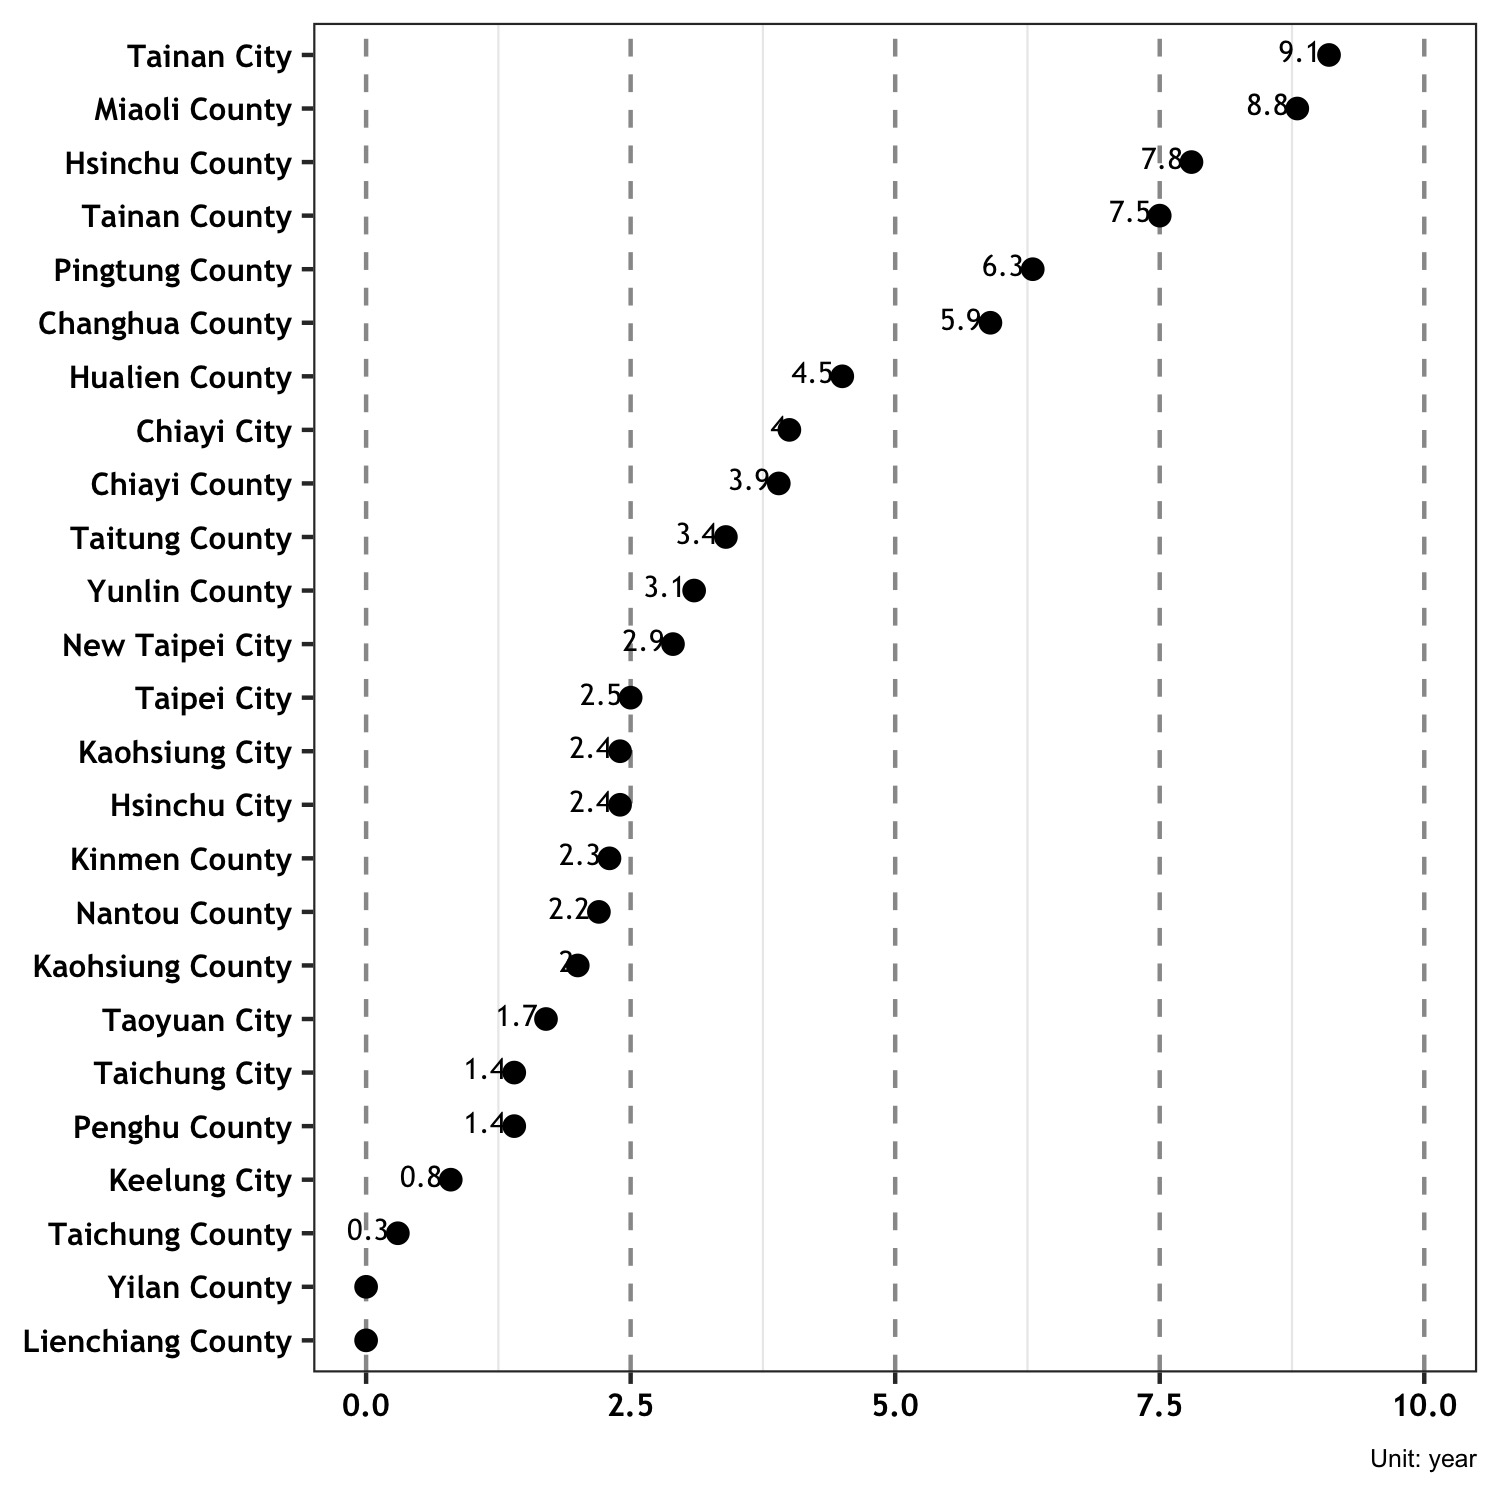
\includegraphics[width=7cm,height=7cm]{04-Chapter-Four/image/figure5-1.jpeg} & 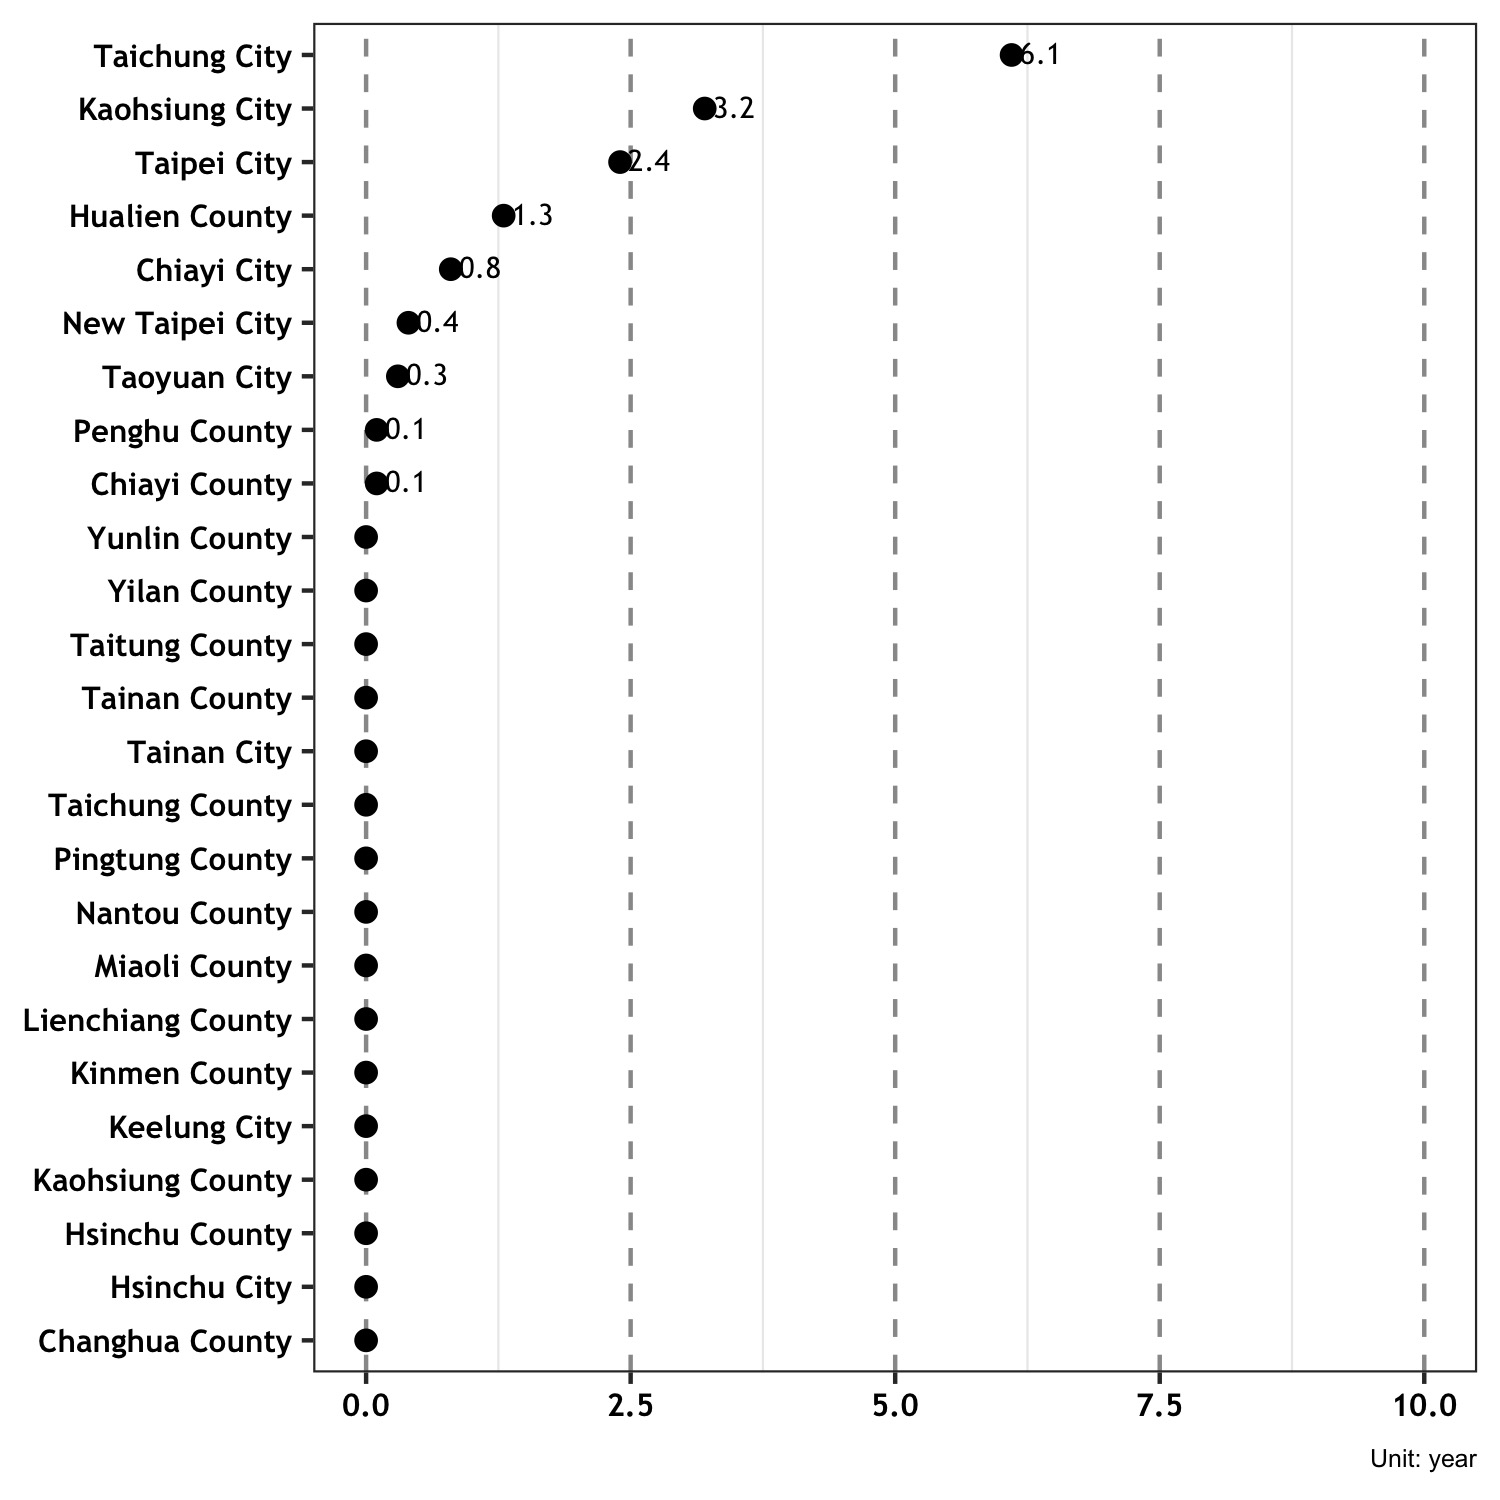
\includegraphics[width=7cm,height=7cm]{04-Chapter-Four/image/figure5-2.jpeg}\tabularnewline
\end{tabular}
Note: This figure depicts the decomposition of the mayor's experience in a pooled mean year.
\end{figure}


\subsection*{Standing Committee Members}


\begin{table}[!htbp]
\caption{The Estimation for the Mayor with Years of Experience \\ 
        as Legislators and Ministers \label{tab:table3}}
\centering{}{\small{}}%
\scalebox{0.85}{
\begin{threeparttable}

\begin{tabular}{lcccc}
\toprule 
\multicolumn{5}{l}{Dependent Variable:}                                                                \\
\multicolumn{5}{l}{\textbf{log (Revenue Support Grant)}}                                               \\
\midrule
                                &  Model (1)      & Model (2)       & Model (3)  & Model (4)          \\
\midrule
$\Delta{\textbf{\textit{ministers}}}$   & 0.267           & 0.514         & 0.682         & 0.046            \\
                                 & 0.364           & 0.406         & 0.418         & 0.348            \\
$\Delta{\textbf{\textit{legislators}}}$ & 0.397$^{***}$   & 0.283         & 0.286         & 0.285$^{*}$      \\
                                 & 0.167           & 0.185         & 0.189         & 0.162            \\
\textbf{standing committee   }                & 0.051           & 0.136$^{***}$ & 0.138$^{**}$  & 0.043            \\
                                 & (0.051)         & (0.059)       & (0.060)       &(0.049)           \\
\textbf{seniority }                          & 0.011           & 0.051         & 0.057         & 0.103            \\
                                 & (0.217)         & (0.177)       & (0.179)       &(0.214)           \\
\textbf{power committee}                  & 0.655$^{***}$   & 0.142         & 0.111         & 0.517$^{***}$.   \\
                                 &(0.117)          & (0.103)       & (0.104)       &(0.121)           \\
\textbf{committee chair}                   & 0.117           & 0.045         & 0.038         & 0.212.           \\
                                 &(0.188)          &(0.150)        & (0.151)       &(0.181)           \\
\textbf{mayoral election}                & 0.017           & 0.018         & 0.020         & 0.385$^{***}$    \\
                                 &(0.055)          &(0.043)        & (0.044)       &(0.104)           \\
\textbf{co-partisan mayors}                & 0.040           & 0.040         & 0.044         & 0.040            \\
                                 &(0.050)          &(0.041)        & (0.041)       &(0.049)           \\
\textbf{\% mayor vote}                      &0.856$^{***}$    & 0.719$^{***}$ & 0.716$^{***}$ & 0.7157$^{***}$   \\
                                 &(0.188)          & (0.1621)      & (0.163)       &(0.183)           \\
\textbf{\% pres. vote}                       & 0.359           & 0.176         & 0.149         & 0.006            \\
                                 & (0.231)         & (0.186)       & (0.188)       &(0.256)           \\
\textbf{co-partisan legislator}           &0.215$^{***}$    & 0.189$^{***}$ & 0.181$^{***}$ & 0.122            \\
                                 &(0.050)          &(0.041)        &(0.041)        &(0.135)           \\
\textbf{\% unemployed}                    & 7.564$^{***}$   & 5.033$^{***}$ & 4.994$^{***}$ &12.940            \\
                                 & (3.518)         & (2.846)       & (2.863)       &(8.312)           \\
\textbf{special cities}                   & 0.692$^{***}$   & 0.102         & 0.078         & 0.703$^{***}$    \\
                                 & (0.067)         & (0.117)       & (0.130)       &(0.064)           \\
\textbf{Constant}                         & 1.938$^{***}$   & 2.053$^{***}$ &               &                  \\
                                 & 0.2067          & 0.197         &               &                  \\
\midrule 
\textbf{No. of observations}             &367              & 367           & 367           & 367              \\
\textbf{adjusted \textit{R}$^{2}$}                   & 0.461           & 0.197         & 0.155         & 0.449            \\
\textbf{model types}                       & Pooled OLS      & RE            & FE            & FE               \\
\textbf{municipality fixed effects }       &                 &               & $\checkmark$  &                  \\
\textbf{fixed effects by year}               &                 &               &               & $\checkmark$     \\
\midrule

\end{tabular}
     \begin{tablenotes}
     Note: * \(p<0.10\),** \(p<0.05\), *** \(p<0.01\). \\ Robust standard errors in parentheses. Standard errors are clustered by municipality. Hausman test\ensuremath{\chi}2 (12)= 13.115 \ensuremath{p}-value = 0.3608 rejects the null hypothesis 
     \end{tablenotes}
     \end{threeparttable}
     }
\end{table}


Following the literature about the importance of legislative committee \citep[e.g.,][]{Martin2014,Wang2013,Hsiao2007, Matsuo2012}, I add another dummy variable as an explanatory variable, \textbf{Standing Committee} in \autoref{tab:table3}, indicating if the mayor has ever had committee membership in the Legislative Yuan. The regression model can be extended as


\begin{equation} \begin{split} \ensuremath{y_{i,t+1}^{grant}}= \ensuremath{\beta_{1}{\Delta minister}_{i,t} +\beta_{2}{\Delta legislator}_{i,t} + \\ \beta_{3}{Standing Committee}_{i,t} +\\ X_{i,t}\gamma + \alpha_{i} + \delta_{t} + \varepsilon_{i,t}}. \end{split} \end{equation} 

Then, I observe some shifts of coefficients in magnitude, especially $\Delta\textit{\textbf{legislators}}$. In column 3 with favoured Random Effect model, \textbf{standing committee} is both statistically and economically significant. This means that when I control for \textbf{standing committee}, a large proportion of significance transfers to this indicator, making it a vital variable in explaining changes in resources among municipalities. Unsurprisingly, the originally significant variable, $\Delta\textit{\textbf{ministers}}$, in \autoref{tab:table3}, is reduced to insignificance.

\begin{figure}[!htbp]
\begin{singlespace}
\begin{centering}
\caption{The Effect of Standing Committee on the Marginal Increase in \\ Revenue Support Grant \label{fig:figure6}}
\par\end{centering}
\end{singlespace}
\begin{centering}
\begin{tabular}{c}
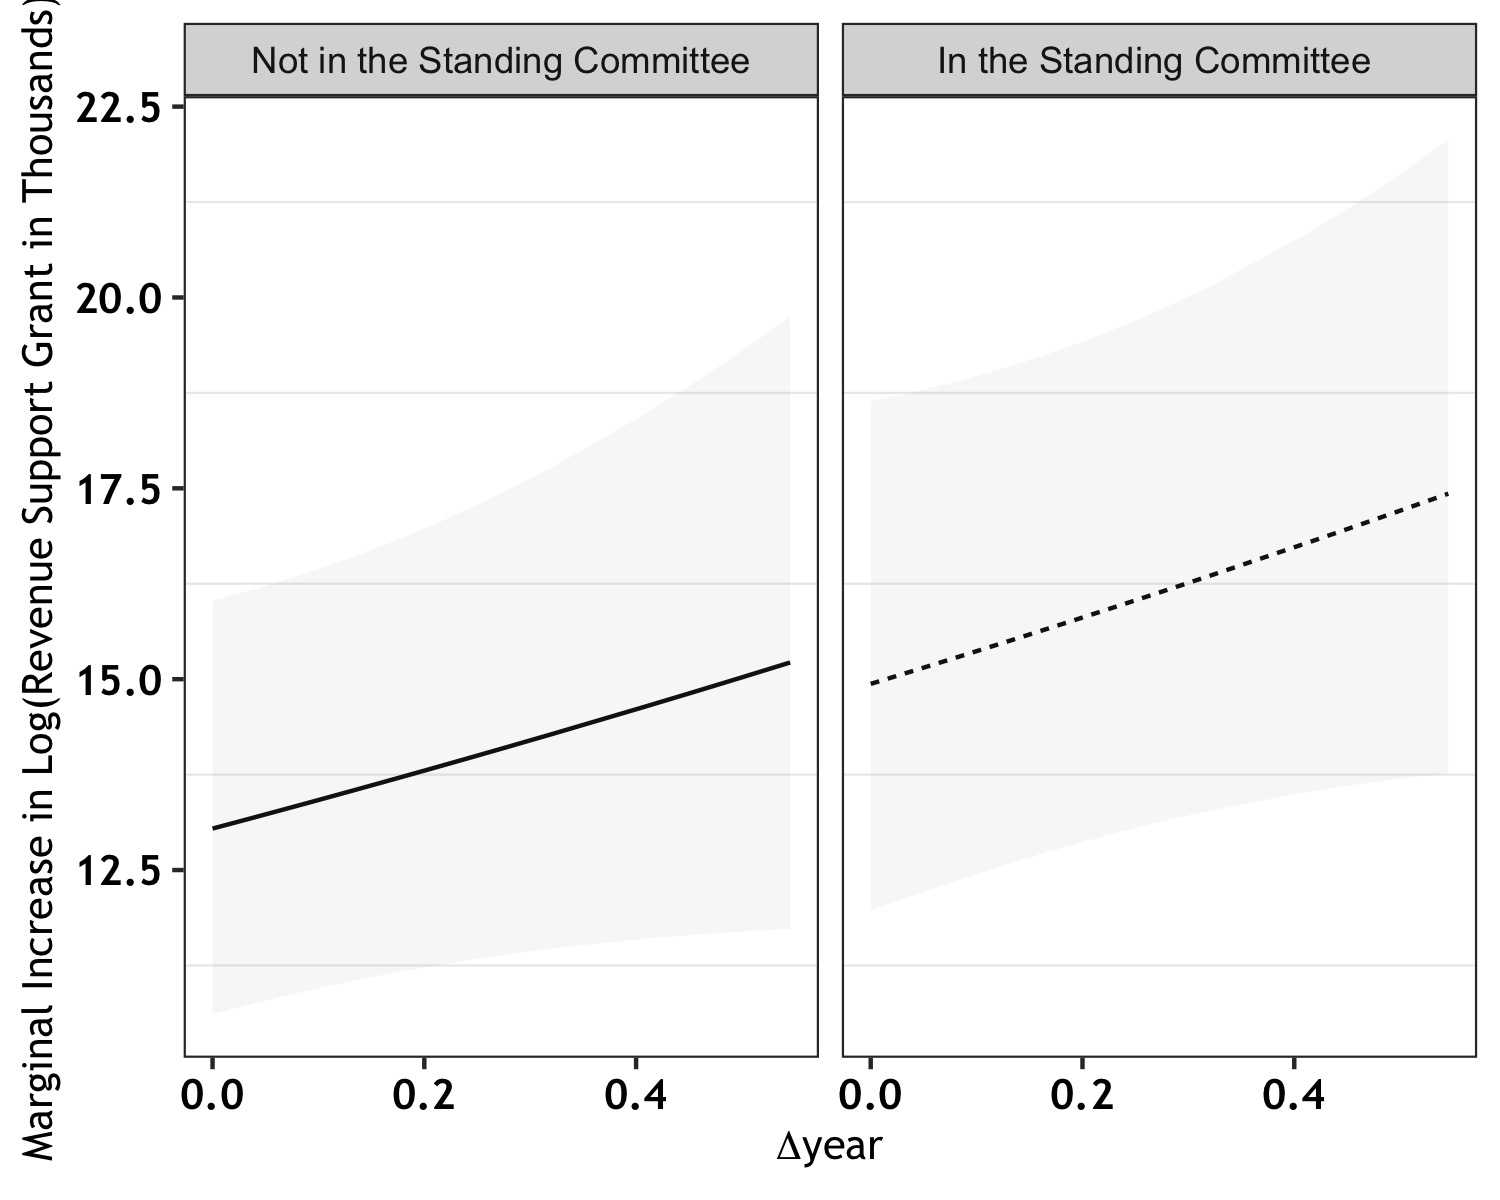
\includegraphics[width=12cm,height=7.5cm]{04-Chapter-Four/image/figure6.jpeg}\tabularnewline
\end{tabular}
\par\end{centering}
Note: The figure present regression coefficients adjusted by all control variables at 95\% percent confidence intervals.
\end{figure}
\textcolor{black}{{} }


This finding suggests that, in explaining the distribution of resources, the effect of $\Delta\ensuremath{legislators}$ is more significant than that of mayors' experience as ministers. More interestingly, the significance of membership in a standing committee even outplays that of the experience as legislators in general, suggesting that the distribution of resources is indeed biased, in favour of municipalities whose mayors served as legislators and among all those mayors with legislator background, prior experience as a standing committee member seems to grant municipalities more privilege in obtaining inter-governmental transferred resources.\footnote{In light of the Hausman test in favour of RE model, I use the estimates from Model (3) in \autoref{tab:table3}.} 

\section*{\centering Conclusion}

Since the emergence of a direct legislative election system in 1992 and a direct presidential election in 1996, central government spending has become inherently susceptible to manipulation for electoral purposes as an inevitable side-effect of such systems. 

The literature on distributive politics has covered various research topics that explain the variation in the distribution of government resources in different contexts and countries. By investigating whether mayors exploit the privilege of being more network-like to the government party to obtain more grants, I identify potential impacts between each mayor's prior years of experience in the central government and the number of financial resources that local government receives. The findings are generally consistent with the literature \citep{Keefer2008,Keefer2009} that a mayor with more connections to the central government obtains substantially more distributive benefits than a political neophyte with less or no political experience.

Finally, while the inequitable distribution of resources is prevalent in most new democracies, the findings are a tentative discovery of the importance of local governments' leaders. I find that municipalities with more years of experience as legislators are allocated more political resources from the central government. The impact is more substantial when mayors have more experience in standing committees.